\documentclass[12pt,letterpaper,oneside]{book}
\usepackage{../afitStyleFiles/afitThesis}
\usepackage{../afitStyleFiles/sf298}
\usepackage[pdftex,pdfpagelabels,bookmarks,hyperindex,hyperfigures]{hyperref}
\hypersetup{
    colorlinks,
    citecolor=black,
    filecolor=black,
    linkcolor=black,
    urlcolor=black
}
\usepackage{float}
\usepackage{tikz}
\usetikzlibrary{positioning}
\usepackage[percent]{overpic}

\mathchardef\mhyphen="2D % Define a "math hyphen"
\graphicspath{{../Figures/}}

\input{Preamble/titlepage}
%% myFigures.tex
% A common file to store all figure definitions
%
% In preparing your thesis, one of the first things you should do is
% organize your figures.  Then, one of the last things you'll do is
% reorder your figures so they display where you want them to in the
% text.  Organizing figure definitions in a common files helps:
%
%   1. Write new figures using earlier examples.
%
%   2.  Isolate code and minimize the risk of introducing bugs in the
%   final editing process.  Trust me, moving around just one line of
%   code is easier.
%
%   3.  Reuse figures in other papers.  <=== the best reason!
%
% Note command names can not include numbers and special characters.
%
% To make the file more searchable, use naming conventions that map
% the graphics filename labSetup.jpg to the command name \figlabSetup to the
% figure label fig:labSetup.
% 

\newcommand{\figproactiveFaultManagement}[1]{\begin{figure}
 \begin{center}
    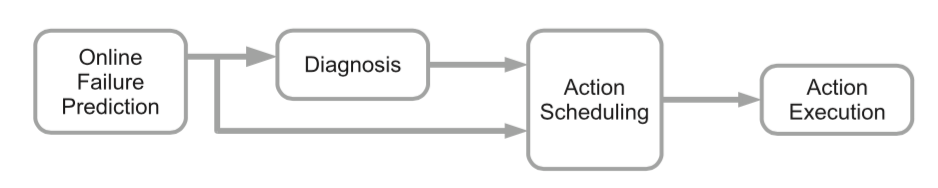
\includegraphics[width=#1]{proactiveFaultManagement}
     \caption[Proactive Fault Management~\cite{salfnerSurvey}]{The stages of
     proactive fault management~\cite{salfnerSurvey}.}
     \label{fig:proactiveFaultManagement}
 \end{center}
\end{figure}
}

\newcommand{\figonlinePrediction}[1]{\begin{figure}
 \begin{center}
    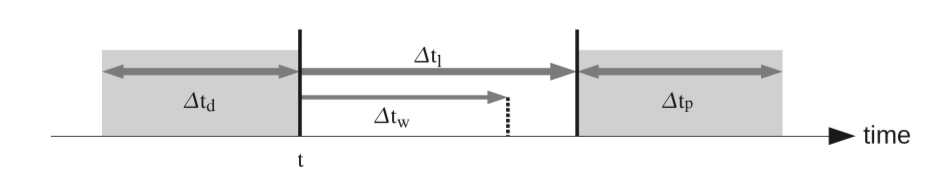
\includegraphics[width=#1]{onlinePrediction}
     \caption[\ac{OFP}~\cite{salfnerSurvey}]{The timeline for
     \ac{OFP}~\cite{salfnerSurvey}.}
     \label{fig:onlinePrediction}
 \end{center}
\end{figure}
}

\newcommand{\figfailureFlowDiagram}[1]{\begin{figure}
 \begin{center}
    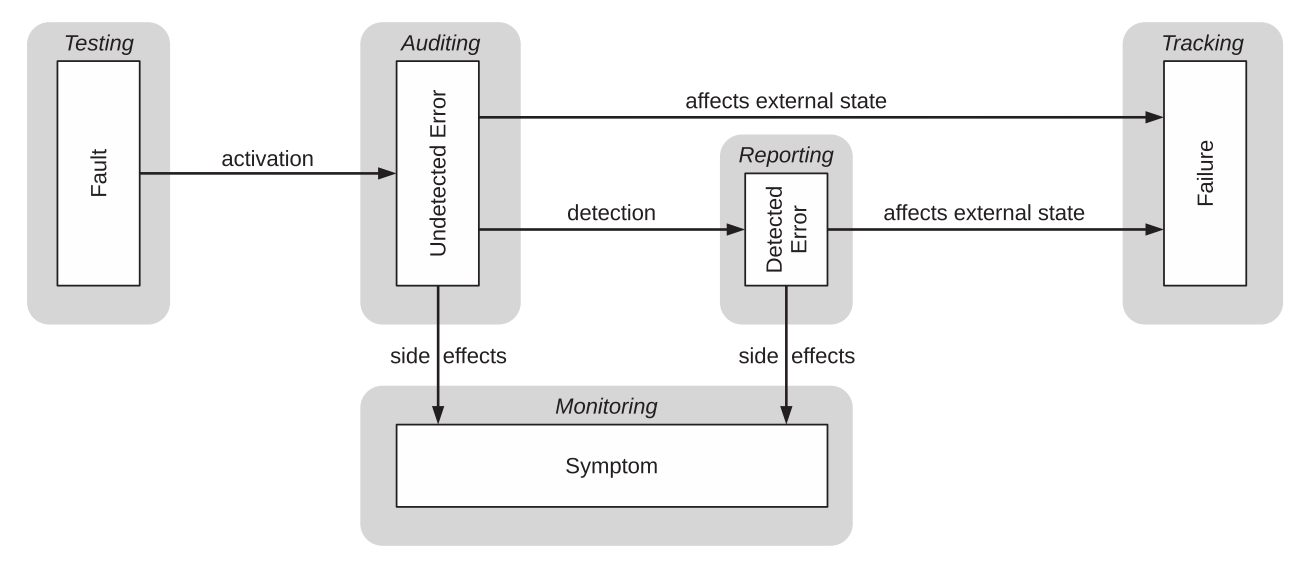
\includegraphics[width=#1]{failureFlowDiagram}
     \caption[Failure Flow Diagram~\cite{salfnerSurvey}]{How faults and errors
     evolve into failure with the associated methods for detection represented
     by enclosing gray boxes~\cite{salfnerSurvey}.}
     \label{fig:failureFlowDiagram}
 \end{center}
 %\vspace{-0.2 in}
\end{figure}
}

\newcommand{\figROC}[1]{\begin{figure}
 \begin{center}
    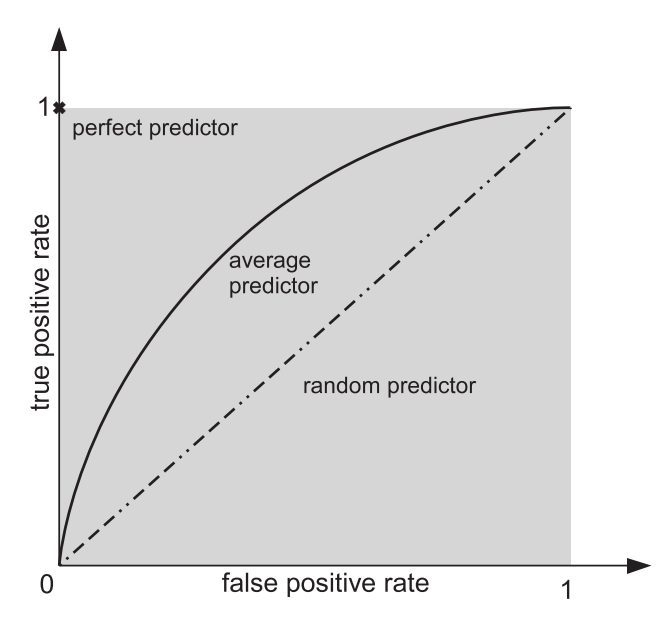
\includegraphics[width=#1]{ROC}
     \caption[Sample \ac{ROC} Plots~\cite{salfnerSurvey}]{\ac{ROC} plots of
     perfect, average, and random predictors~\cite{salfnerSurvey}.}
     \label{fig:ROC}
 \end{center}
\end{figure}
}

\newcommand{\figprecisionRecallCurve}[1]{\begin{figure}
 \begin{center}
    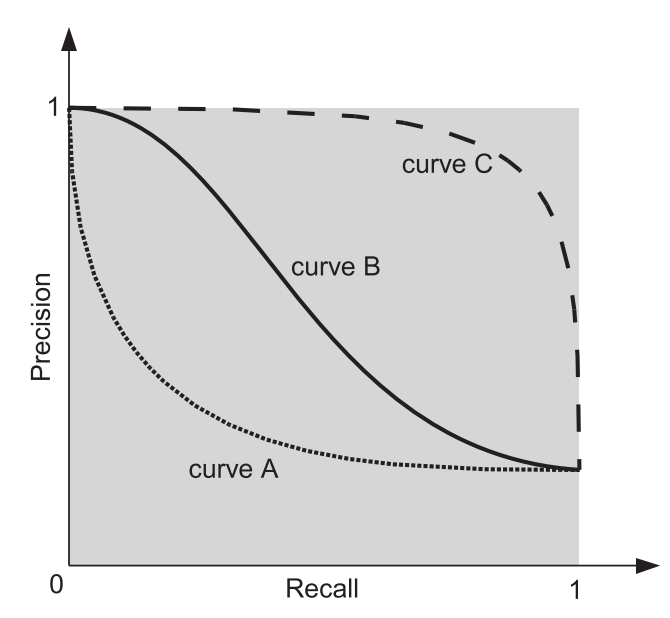
\includegraphics[width=#1]{precisionRecallCurve}
     \caption[Sample Precision/Recall Curves~\cite{salfnerSurvey}]{Sample
     precision/recall curves~\cite{salfnerSurvey}.  Curve $A$ represents a
     poorly performing predictor, curve $B$ an average predictor, and curve $C$
     an exceptional predictor.}
     \label{fig:precisionRecallCurve}
 \end{center}
\end{figure}
}

\newcommand{\figpatternRecognition}[1]{\begin{figure}
 \begin{center}
    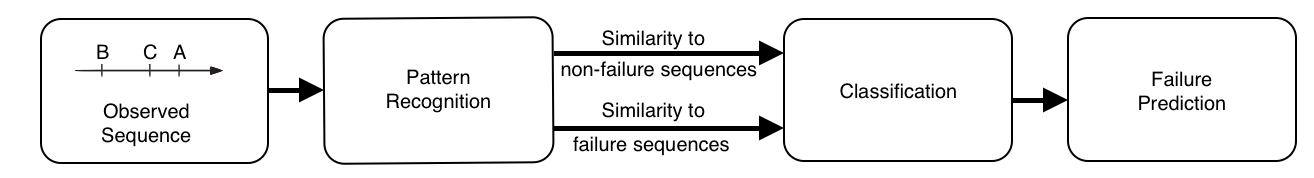
\includegraphics[width=#1]{patternRecognition}
     \caption[Pattern recognition in reported errors~\cite{salfnerSurvey}]{How
     pattern recognition is accomplished in reported
     errors~\cite{salfnerSurvey}.}
     \label{fig:patternRecognition}
 \end{center}
\end{figure}
}

\newcommand{\figAFP}[1]{\begin{figure}[t!h]
 \begin{center}
    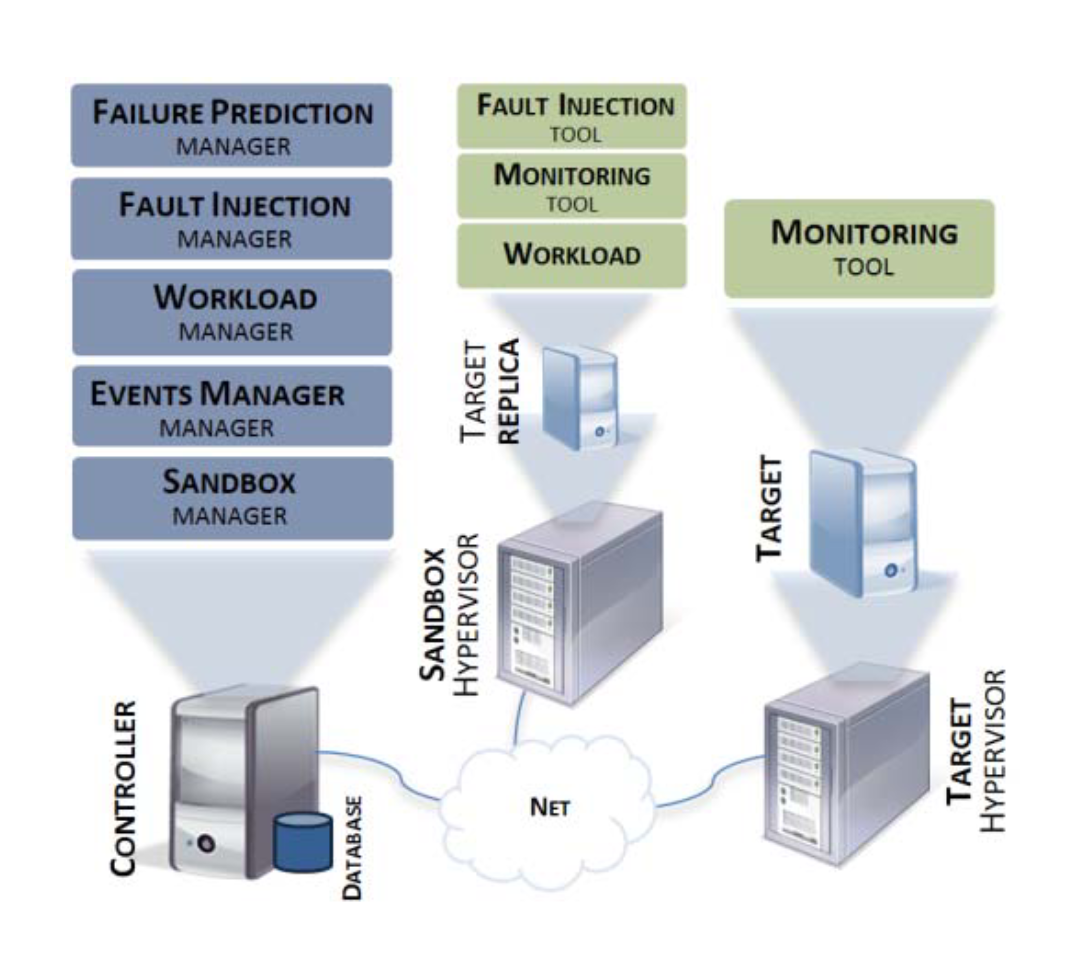
\includegraphics[width=#1]{AFP}
     \caption{The \ac{AFP} framework~\cite{irrera2015}.}
     \label{fig:AFP}
 \end{center}
\end{figure}
}

\definecolor{airforceblue}{rgb}{0.36, 0.54, 0.66}
\definecolor{armygreen}{rgb}{0.29, 0.33, 0.13}

\newcommand{\figannotatedAFPcolor}{\begin{figure}
 \begin{center}
     \begin{overpic}[width=5in,scale=.25]{annotatedAFPcolor}
       \put(8,0){
         \begin{tikzpicture}
           [node font=\footnotesize, label/.style={rectangle, draw,
           fill=airforceblue, text width=2cm, text badly centered, minimum
           height=0.5cm, rounded corners}]

           \node[label] (FPMgr)
             {\textcolor{white}{\ref{sec:failurePrediction}}};
           \node[label, below=1.2cm of FPMgr] (FIMgr) 
             {\textcolor{white}{\ref{sec:faultInjectionMgr}}};
           \node[label, below=1.3cm of FIMgr] (WMgr) 
             {\textcolor{white}{\ref{sec:workloadMgr}}};
           \node[label, below=1.2cm of WMgr] (EMMgr) 
             {\textcolor{white}{\ref{sec:eventsManagerMgr}}};
           \node[label, below=1.2cm of EMMgr] (SMgr) 
             {\textcolor{white}{\ref{sec:sandboxMgr}}};
           \node[label, below=4.75cm of SMgr] (Controller) 
             {\textcolor{white}{\ref{sec:controller}}};
         \end{tikzpicture}
       }

       \put(40,60.5){
         \begin{tikzpicture}
           [node font=\footnotesize, label/.style={rectangle, draw,
           fill=armygreen, text width=2cm, text badly centered, minimum
           height=0.5cm, rounded corners}]

           \node[label] (Sandbox)
             {\textcolor{white}{\ref{sec:sandbox}}};
           \node[label, below=1.2cm of Sandbox] (SBFITool)
             {\textcolor{white}{\ref{sec:faultInjectionTool}}};
           \node[label, below=0.95cm of SBFITool] (SBMTool) 
             {\textcolor{white}{\ref{sec:sandboxMonitoringTool}}};
           \node[label, below=0.95cm of SBMTool] (SBWorkload) 
             {\textcolor{white}{\ref{sec:sandboxWorkload}}};
         \end{tikzpicture}
       }

       \put(66,0){
         \begin{tikzpicture}
           [node font=\footnotesize, label/.style={rectangle, draw,
           fill=armygreen, text width=2cm, text badly centered, minimum
           height=0.5cm, rounded corners}]

           \node[label] (MonTool)
             {\textcolor{white}{\ref{sec:targetMonitoringTool}}};
           \node[label, below=7.85cm of MonTool] (Target)
             {\textcolor{white}{\ref{sec:target}}};
         \end{tikzpicture}
       }
     \end{overpic}
     \caption[Annotated \ac{AFP} Framework~\cite{irrera2015}]{The \ac{AFP}
     framework implementation~\cite{irrera2015} with modified components
     highlighted.}
     \label{fig:annotatedAFP}
 \end{center}
\end{figure}
}

\newcommand{\figannotatedAFP}{\begin{figure}
 \begin{center}
     \begin{overpic}[width=5in,scale=.25]{annotatedAFP}
       \put(8,0){
         \begin{tikzpicture}
           [node font=\footnotesize, label/.style={rectangle, draw,
           fill=white, text width=2cm, text badly centered, minimum
           height=0.5cm, rounded corners}]

           \node[label] (FPMgr)
             {\textcolor{black}{\ref{sec:failurePrediction}}};
           \node[label, below=1.2cm of FPMgr] (FIMgr) 
             {\textcolor{black}{\ref{sec:faultInjectionMgr}}};
           \node[label, below=1.3cm of FIMgr] (WMgr) 
             {\textcolor{black}{\ref{sec:workloadMgr}}};
           \node[label, below=1.2cm of WMgr] (EMMgr) 
             {\textcolor{black}{\ref{sec:eventsManagerMgr}}};
           \node[label, below=1.2cm of EMMgr] (SMgr) 
             {\textcolor{black}{\ref{sec:sandboxMgr}}};
           \node[label, below=4.75cm of SMgr] (Controller) 
             {\textcolor{black}{\ref{sec:controller}}};
         \end{tikzpicture}
       }

       \put(40,60.5){
         \begin{tikzpicture}
           [node font=\footnotesize, label/.style={rectangle, draw,
           fill=white, text width=2cm, text badly centered, minimum
           height=0.5cm, rounded corners}]

           \node[label] (Sandbox)
             {\textcolor{black}{\ref{sec:sandbox}}};
           \node[label, below=1.2cm of Sandbox] (SBFITool)
             {\textcolor{black}{\ref{sec:faultInjectionTool}}};
           \node[label, below=0.95cm of SBFITool] (SBMTool) 
             {\textcolor{black}{\ref{sec:sandboxMonitoringTool}}};
           \node[label, below=0.95cm of SBMTool] (SBWorkload) 
             {\textcolor{black}{\ref{sec:sandboxWorkload}}};
         \end{tikzpicture}
       }

       \put(66,0){
         \begin{tikzpicture}
           [node font=\footnotesize, label/.style={rectangle, draw,
           fill=white, text width=2cm, text badly centered, minimum
           height=0.5cm, rounded corners}]

           \node[label] (MonTool)
             {\textcolor{black}{\ref{sec:targetMonitoringTool}}};
           \node[label, below=7.85cm of MonTool] (Target)
             {\textcolor{black}{\ref{sec:target}}};
         \end{tikzpicture}
       }
     \end{overpic}
     \caption[Annotated \ac{AFP} Framework~\cite{irrera2015}]{The \ac{AFP}
     framework implementation~\cite{irrera2015} with modified components
     highlighted.}
     \label{fig:annotatedAFP}
 \end{center}
\end{figure}
}

\newcommand{\figTrainingPhase}[1]{\begin{figure}[h!t]
 \begin{center}
  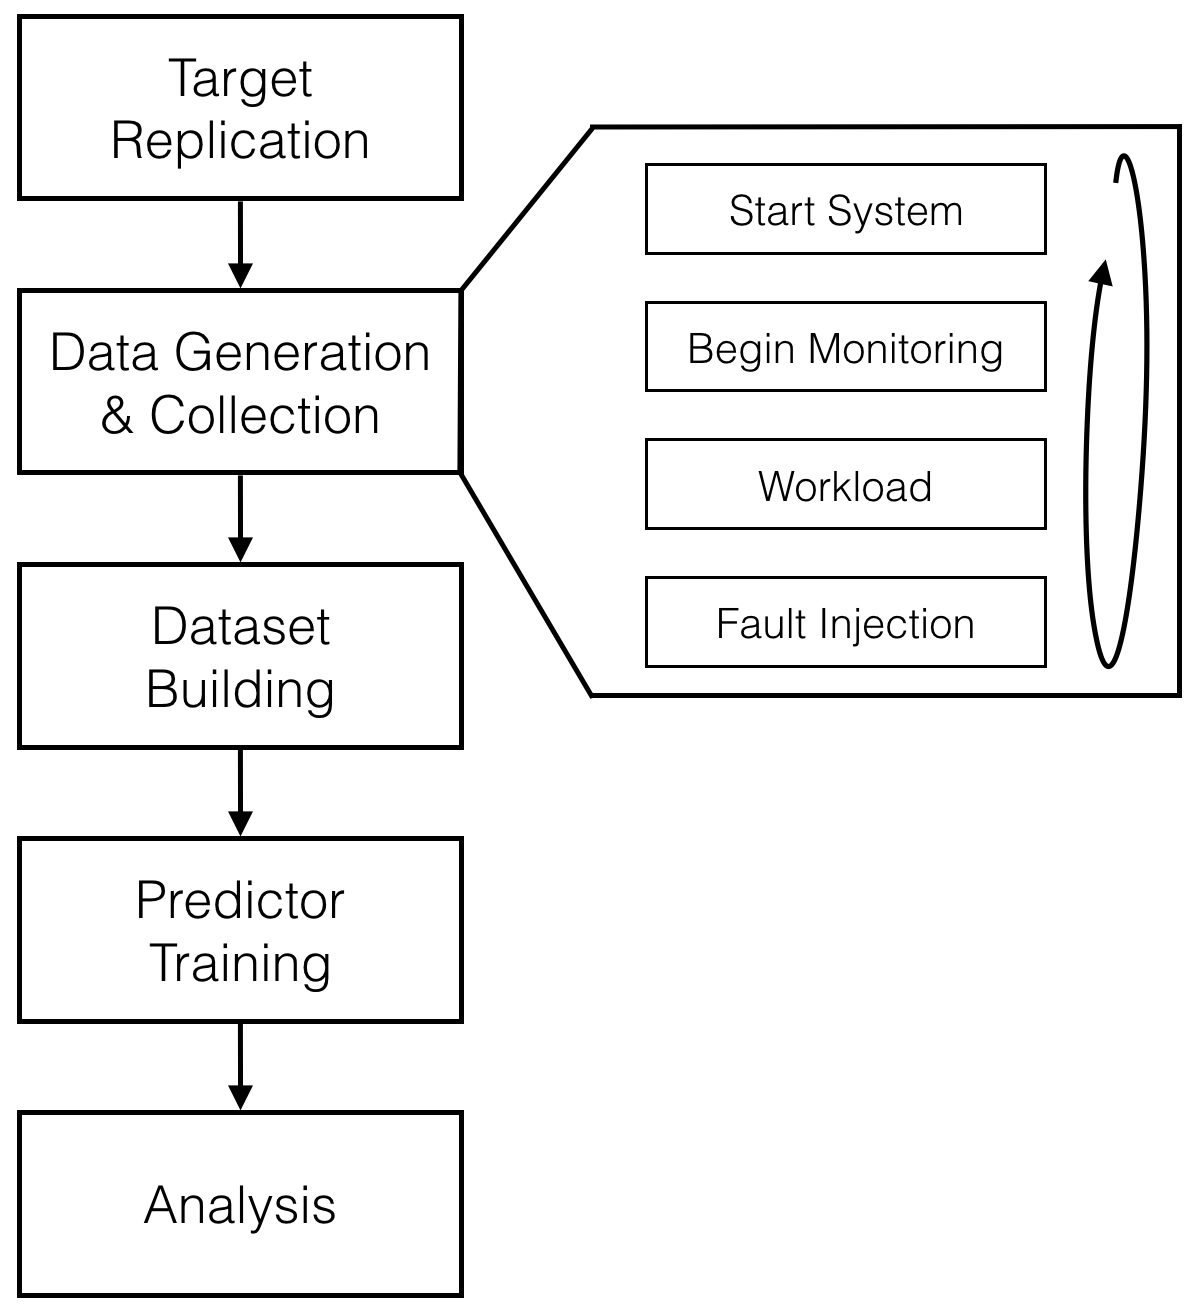
\includegraphics[width=#1]{TrainingPhase}
  \caption[\ac{AFP} Training Phase~\cite{irrera2015}]{The flow of the major
  steps involved in the \ac{AFP} framework training phase~\cite{irrera2015}.}
  \label{fig:TrainingPhase}
 \end{center}
\end{figure}
}

\newcommand{\figExecutionPhase}[1]{\begin{figure}[h!t]
  \begin{center}
    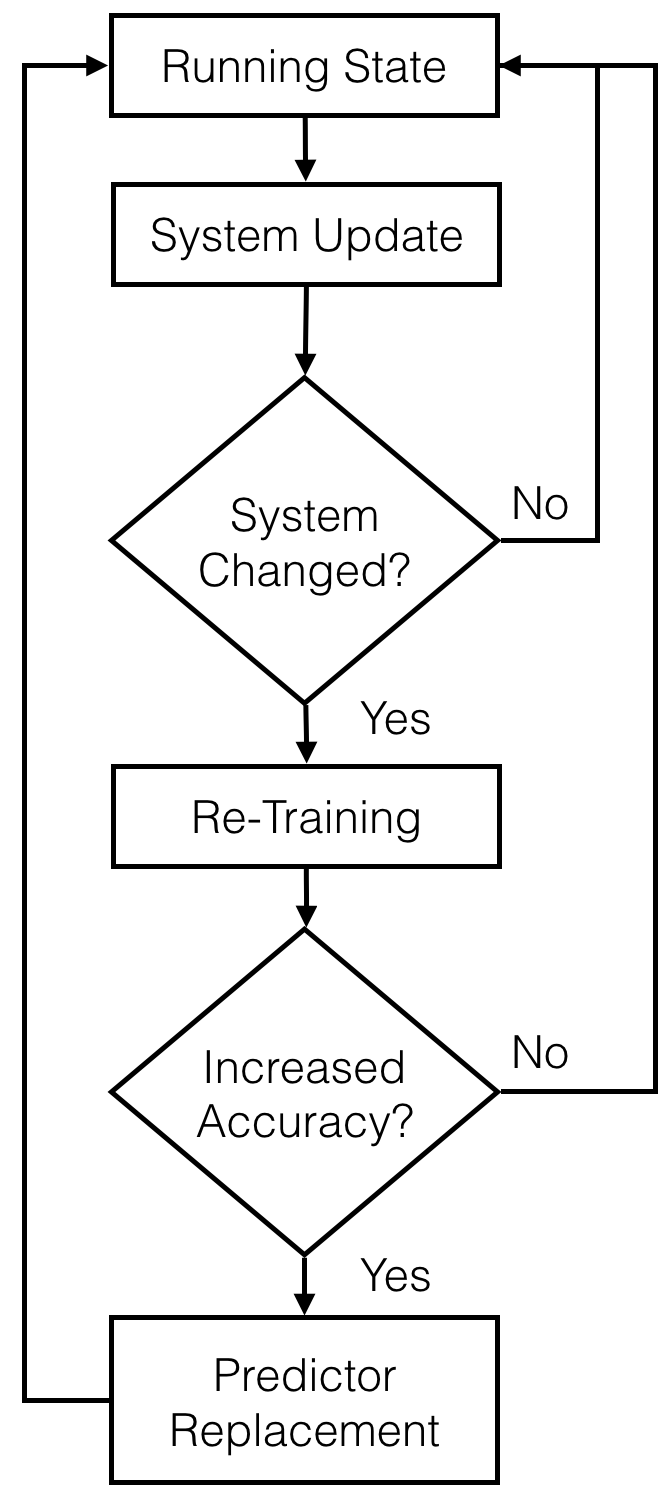
\includegraphics[width=#1]{ExecutionPhase}
    \caption[\ac{AFP} Execution Phase~\cite{irrera2015}]{The flow of the major
    steps involved in the \ac{AFP} framework execution
    phase~\cite{irrera2015}.}
    \label{fig:ExecutionPhase}
  \end{center}
\end{figure}
}


\newcommand{\figExecutionPhaseHoriz}[1]{\begin{figure}
  \begin{center}
    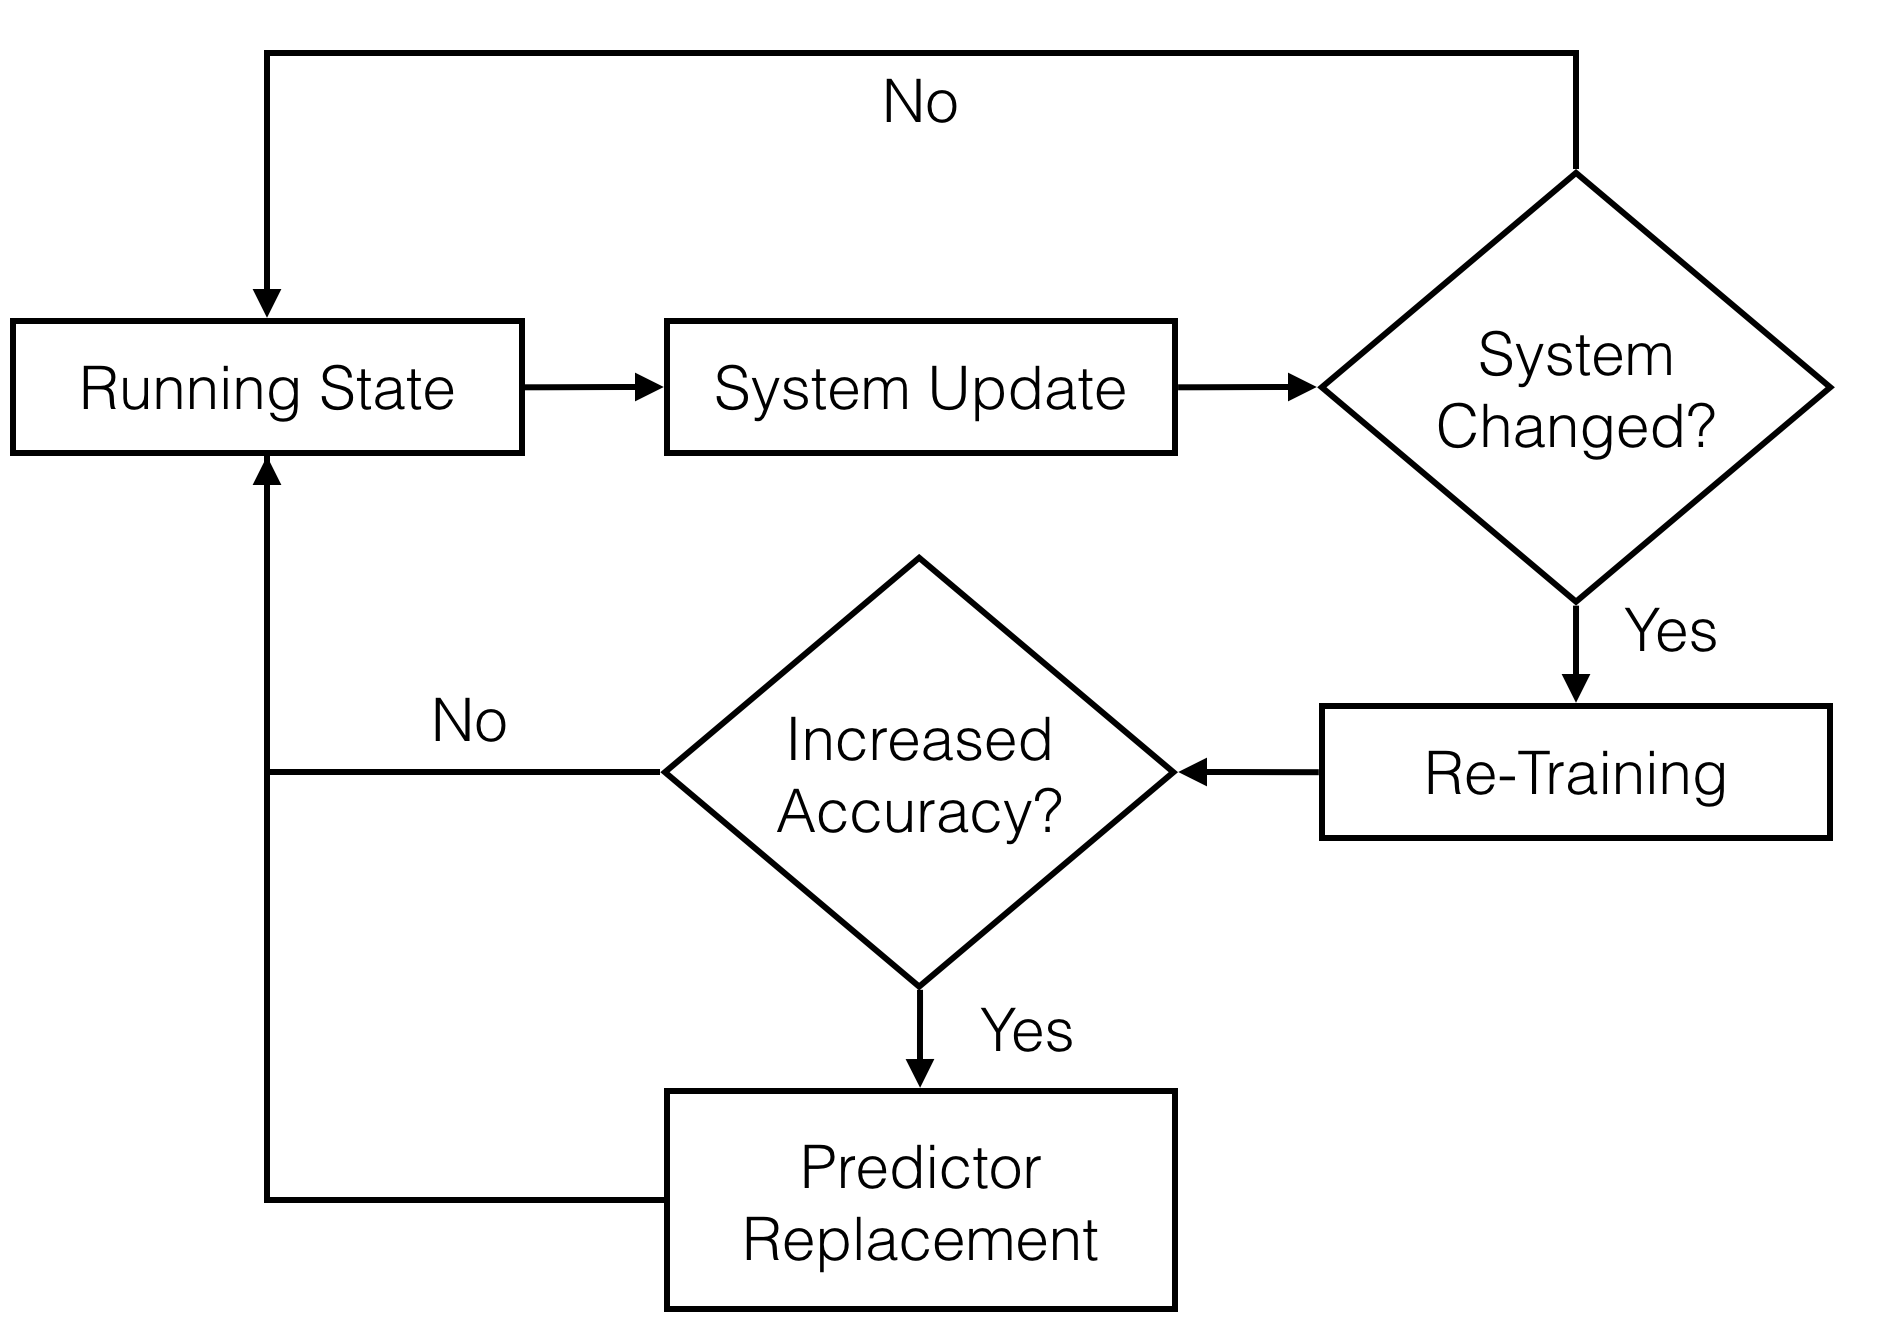
\includegraphics[width=#1]{ExecutionPhaseHoriz}
    \caption[\ac{AFP} Execution Phase~\cite{irrera2015}]{The flow of the major
    steps involved in the \ac{AFP} framework execution
    phase~\cite{irrera2015}.}
    \label{fig:ExecutionPhaseHoriz}
  \end{center}
\end{figure}
}

\newcommand{\figAuthDCPPS}[1]{\begin{figure}
 \begin{center}
  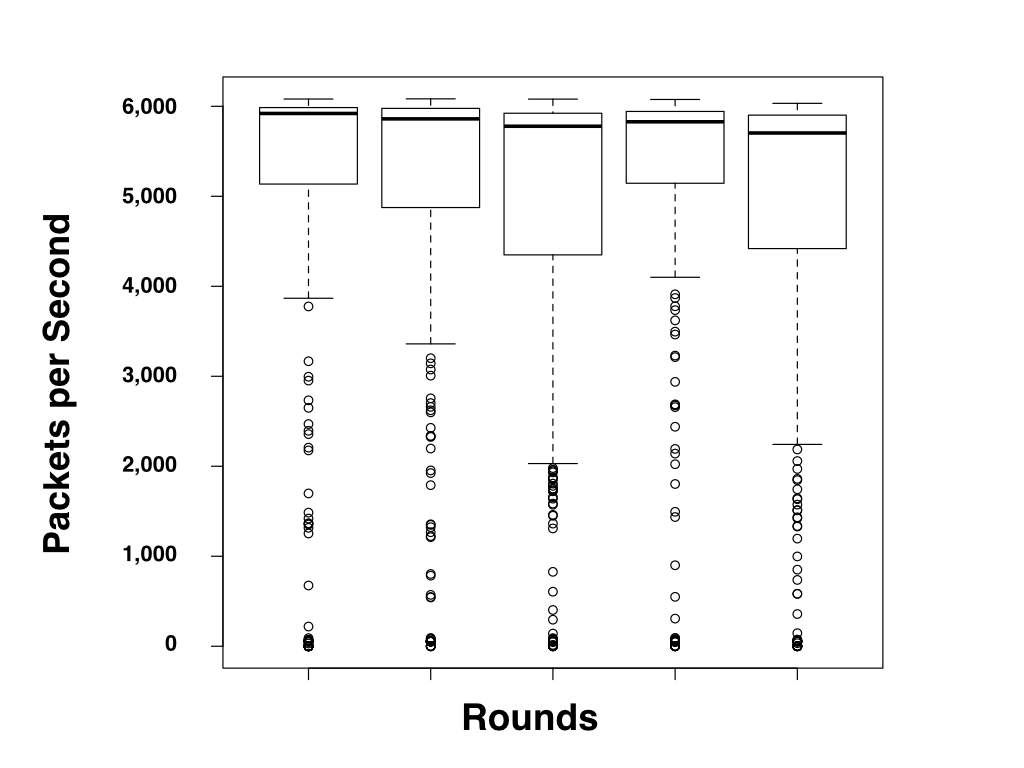
\includegraphics[width=#1]{DPLG/authDCPPS}
  \caption[Domain Controller Packets per Second]{How many packets per second
  were sent or received by the domain controller across all five rounds of the
  first test.  In each test, we captured approximately 1.8 million packets.}
  \label{fig:authDCPPS}
 \end{center}
\end{figure}
}

\newcommand{\figAuthClientPPS}[1]{\begin{figure}
 \begin{center}
  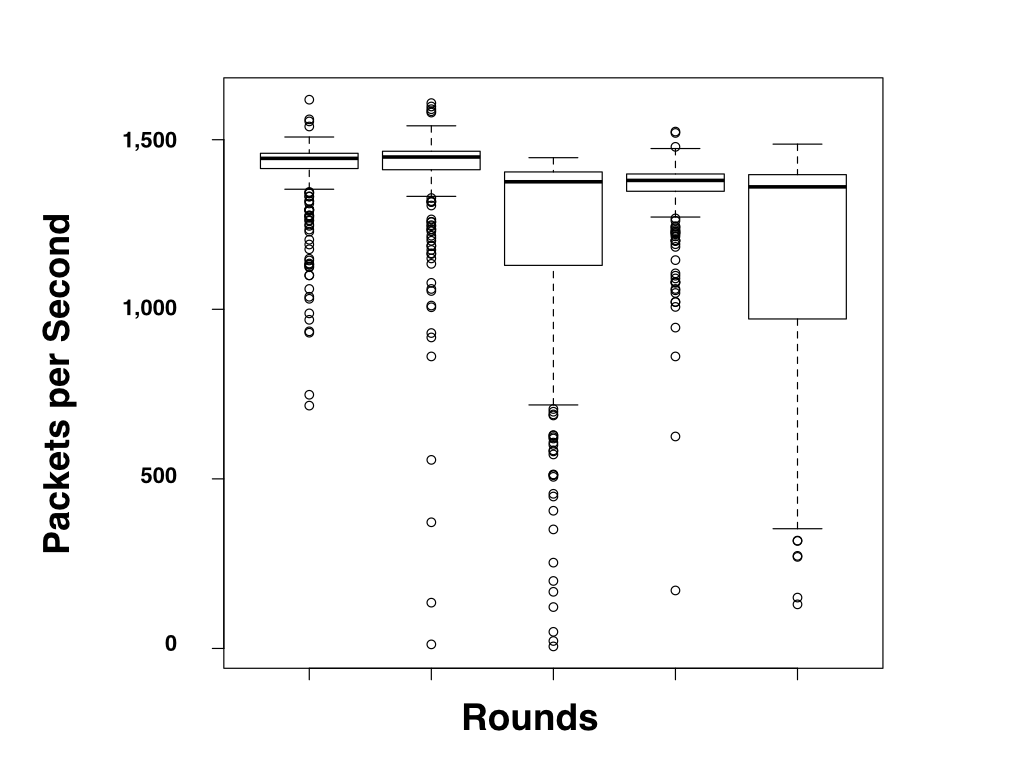
\includegraphics[width=#1]{DPLG/authClientPPS}
  \caption[Client Packets per Second]{How many packets per second were sent or
  received by one of the clients across all five rounds of the first test.}
  \label{fig:authClientPPS}
 \end{center}
\end{figure}
}

\newcommand{\figAuthDCMetrics}[1]{\begin{figure}
 \begin{center}
  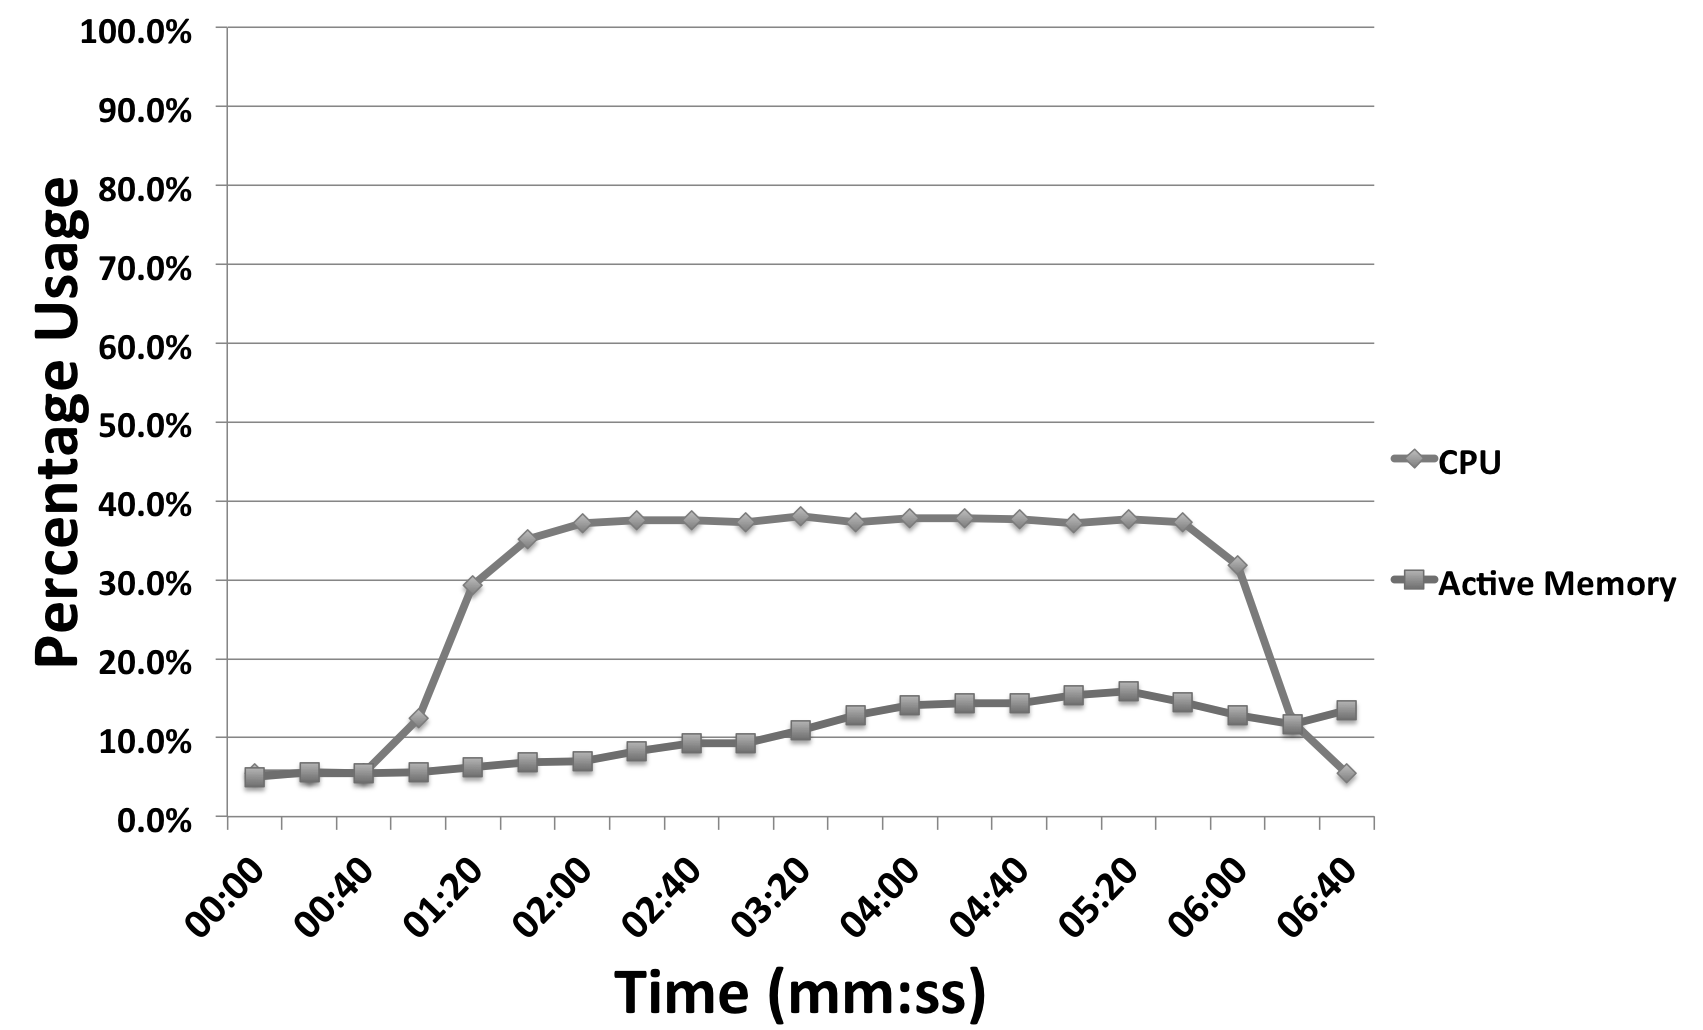
\includegraphics[width=#1]{DPLG/authDCMetrics}
  \caption[Test 1:  Domain Controller Performance]{Domain controller CPU and
  memory utilization during the first test.}
  \label{fig:authDCMetrics}
 \end{center}
\end{figure}
}

\newcommand{\figOFPTaxonomy}[1]{\begin{figure}
 \begin{center}
  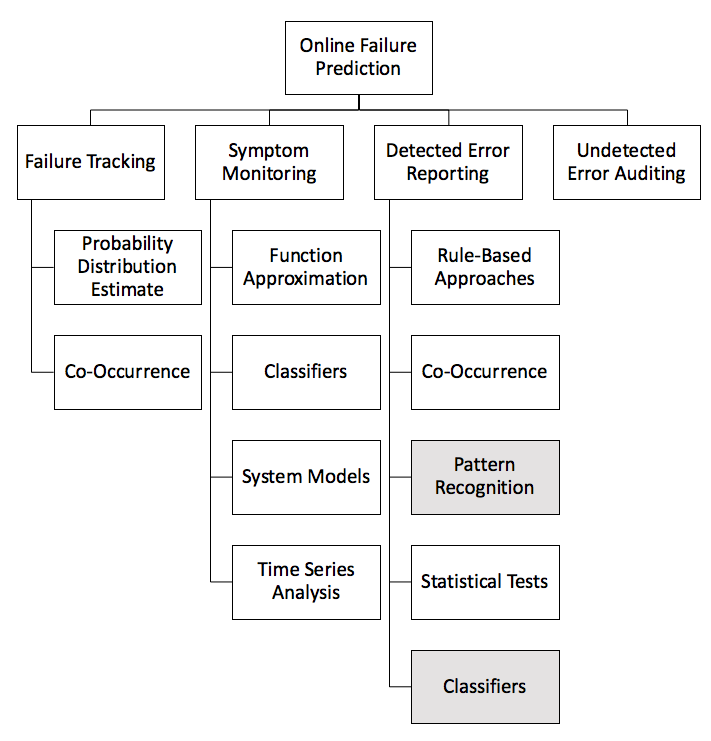
\includegraphics[width=#1]{OFPTaxonomy}
  \caption[Taxonomy of \ac{OFP} Approaches]{Taxonomy of approaches to online
  failure prediction~\cite{salfnerSurvey}.  The two categories into which this
  research falls are highlighted.}
  \label{fig:OFPTaxonomy}
 \end{center}
\end{figure}
}

\newcommand{\figMemLeakROC}[1]{\begin{figure}
 \begin{center}
  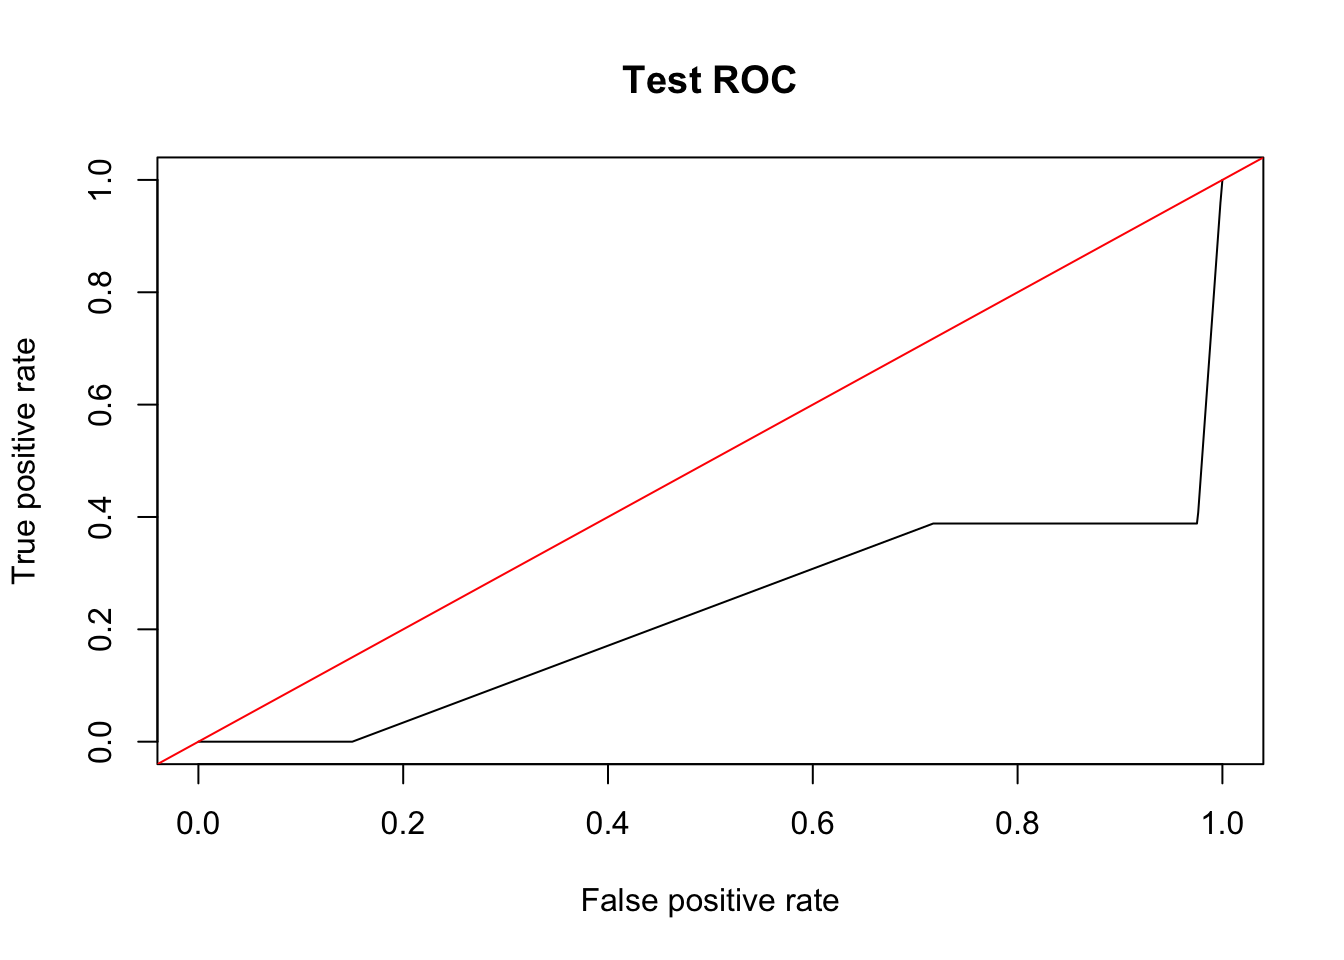
\includegraphics[width=#1]{MemLeakROC}
  \caption[\ac{SVM} Memory Leak \ac{ROC} Curve]{\ac{SVM} memory leak test data
  \ac{ROC} curve.}
  \label{fig:memLeakROC}
 \end{center}
\end{figure}
}

\newcommand{\figMemLeakCompare}[1]{\begin{figure}
 \begin{center}
  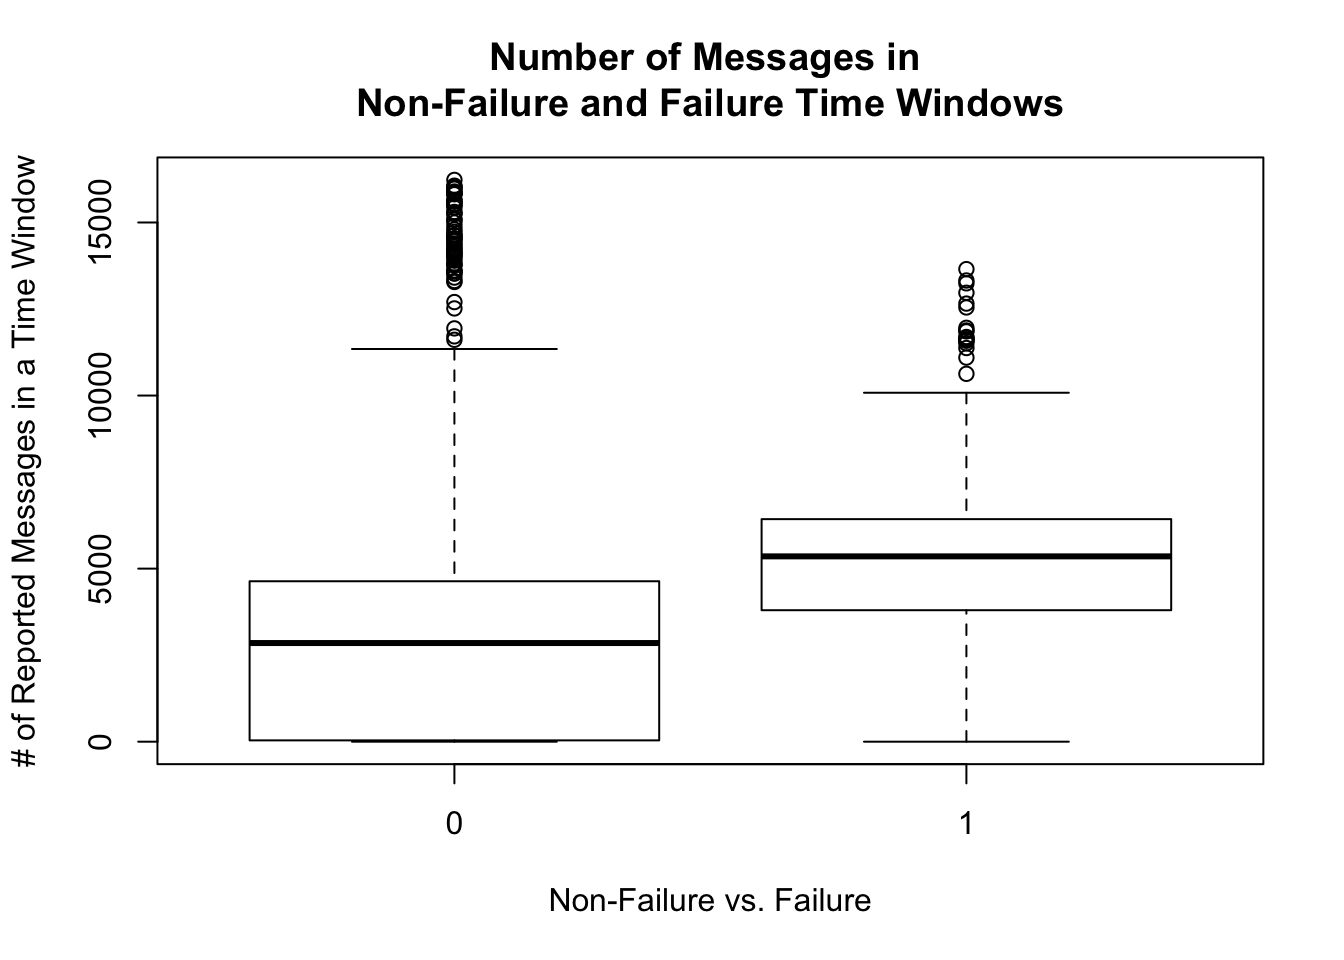
\includegraphics[width=#1]{MemLeakCompare}
  \caption[\ac{SVM} Memory Leak Performance Comparison]{Number of observations
  in a given thirty second time window where `1' represents a window during
  which failure occurred and `0' represents a window during which no failure
  occurred.}
  \label{fig:memLeakCompare}
 \end{center}
\end{figure}
}

%%%%   SMV   %%%%
% Pre-Update
\newcommand{\figMemLeakPreUpdateSVMPerf}{\begin{figure*}
  \centering
  \subfigure[Precision/Recall Curve.]{
    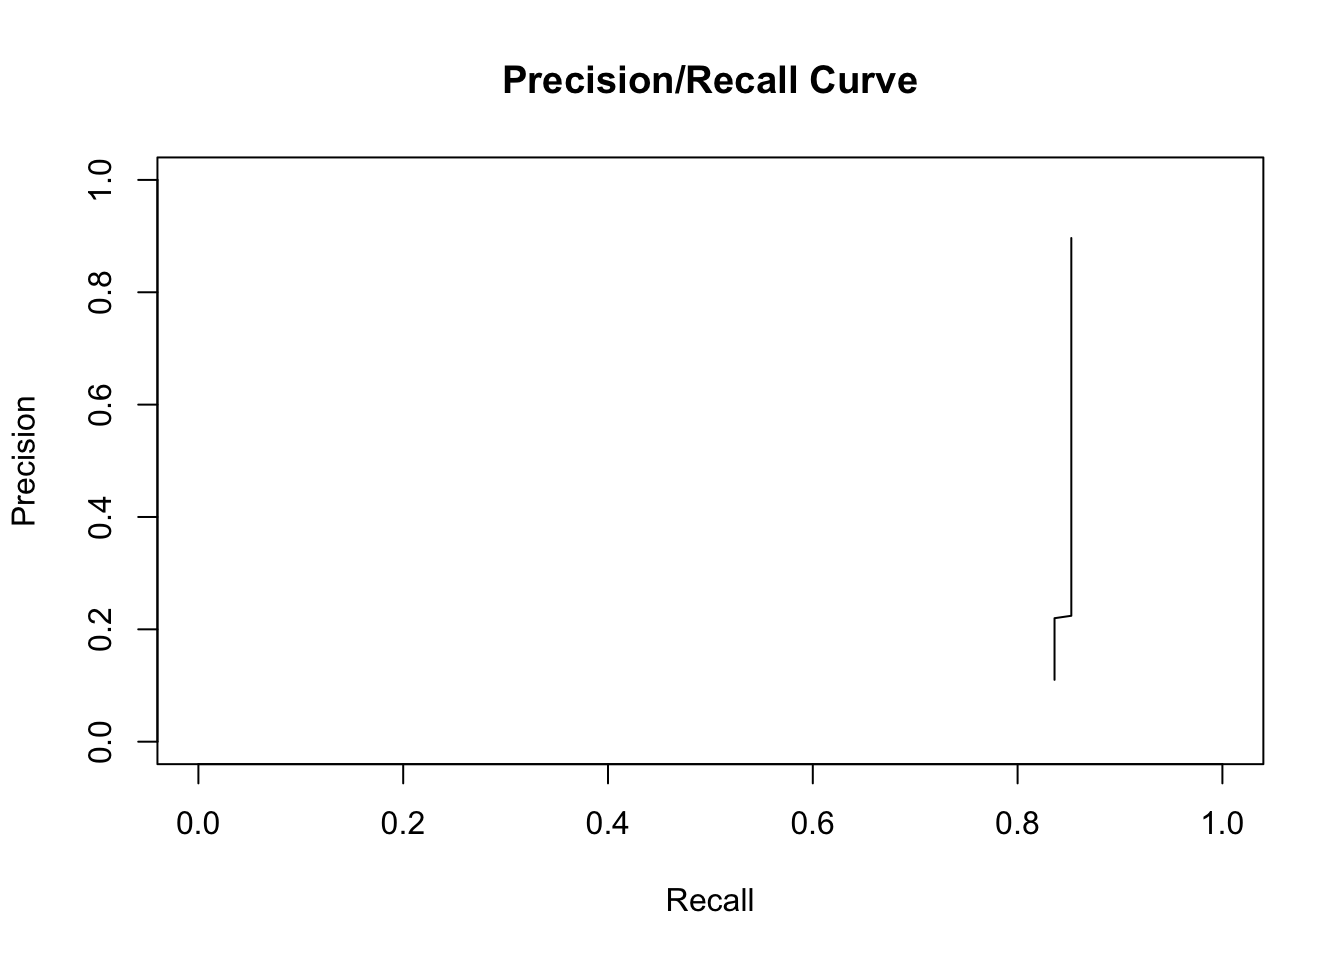
\includegraphics[width=0.45\textwidth]{results/pre-update/memleak/svm-prc}
  }
  \subfigure[\ac{ROC} Curve (\ac{AUC} = 0.8664).]{
    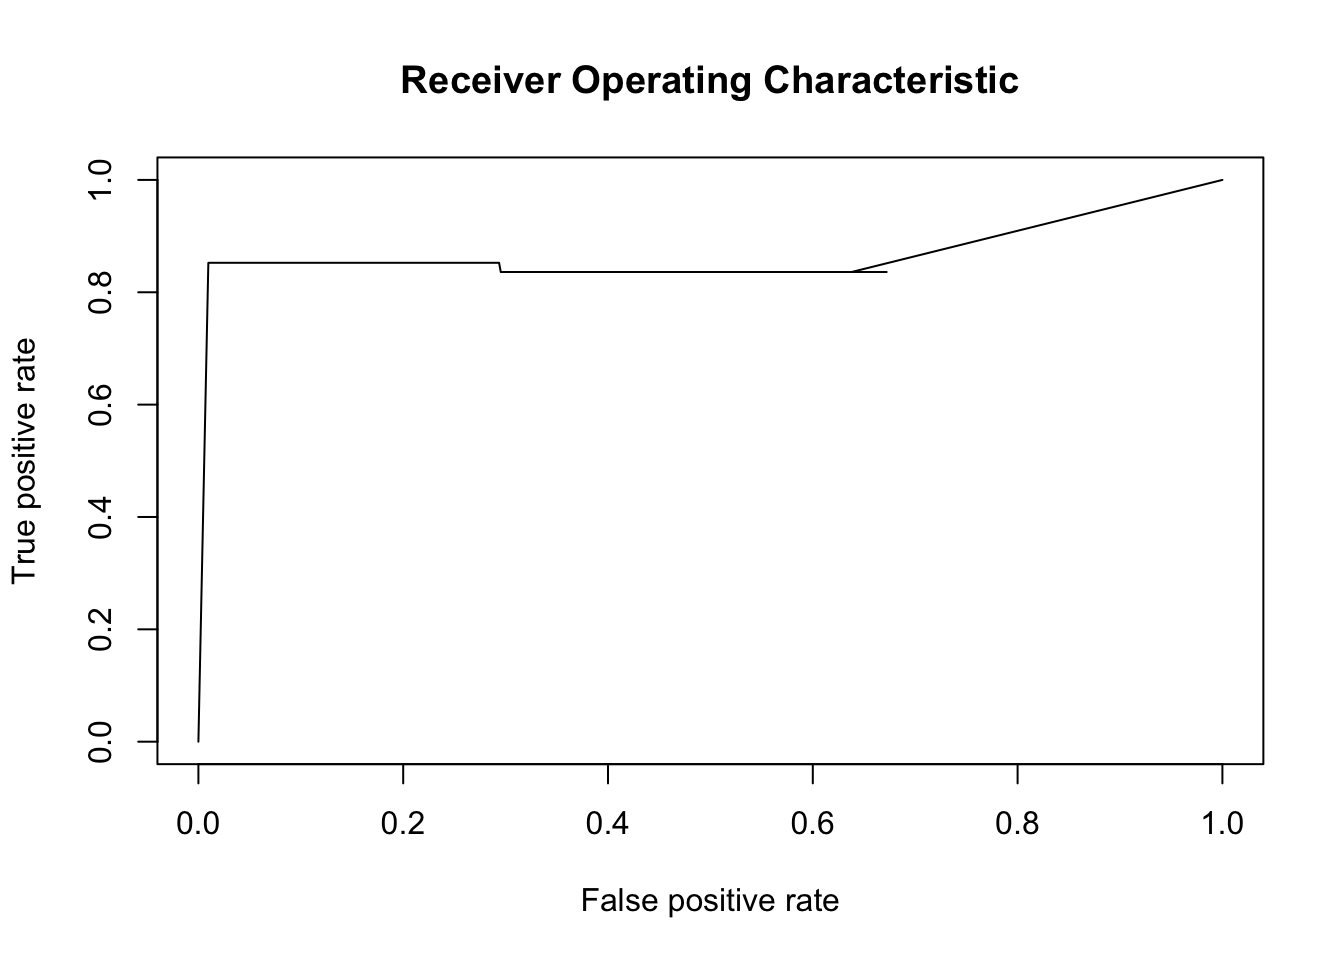
\includegraphics[width=0.45\textwidth]{results/pre-update/memleak/svm-roc}
  }
  \caption[Pre-Update, Memory Leak \ac{SVM} Performance]{Test data performance
  of the \ac{SVM} prediction method on failure data obtained by consuming all
  available memory until target application fails.}
  \label{fig:memLeakPreUpdateSVMPerf}
\end{figure*}
}

% Post-Update (old model)

% Post-Update New Model

%%%%   BOOSTING   %%%%
% Pre-Update
\newcommand{\figMemLeakPreUpdateBoostingPerf}{\begin{figure*}
  \centering
  \subfigure[Precision/Recall Curve.]{
    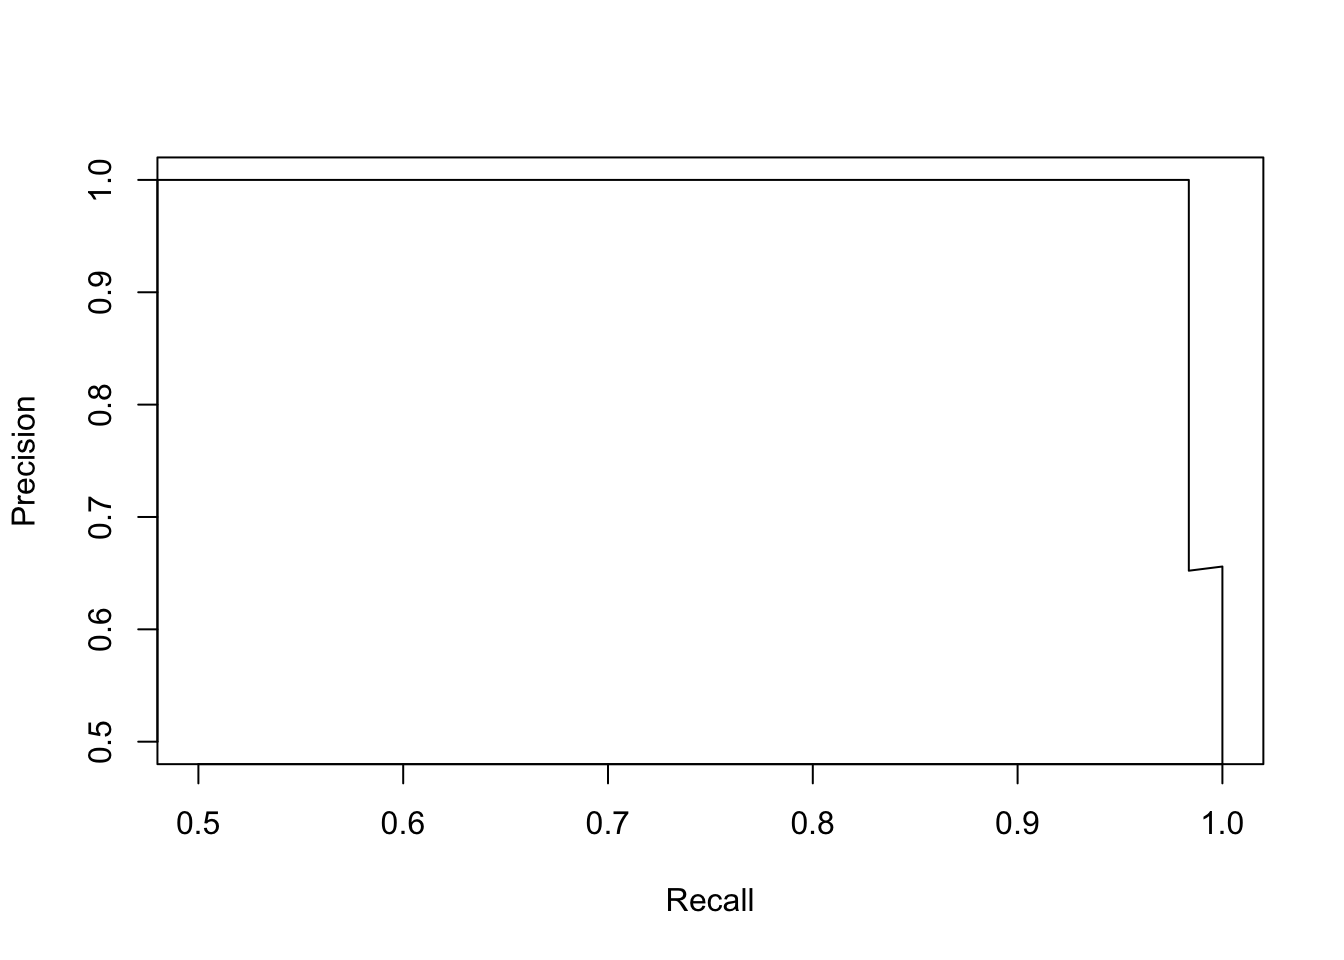
\includegraphics[width=0.45\textwidth]{results/pre-update/memleak/boosting-prc}
  }
  \subfigure[\ac{ROC} Curve (\ac{AUC} = 0.9984).]{
    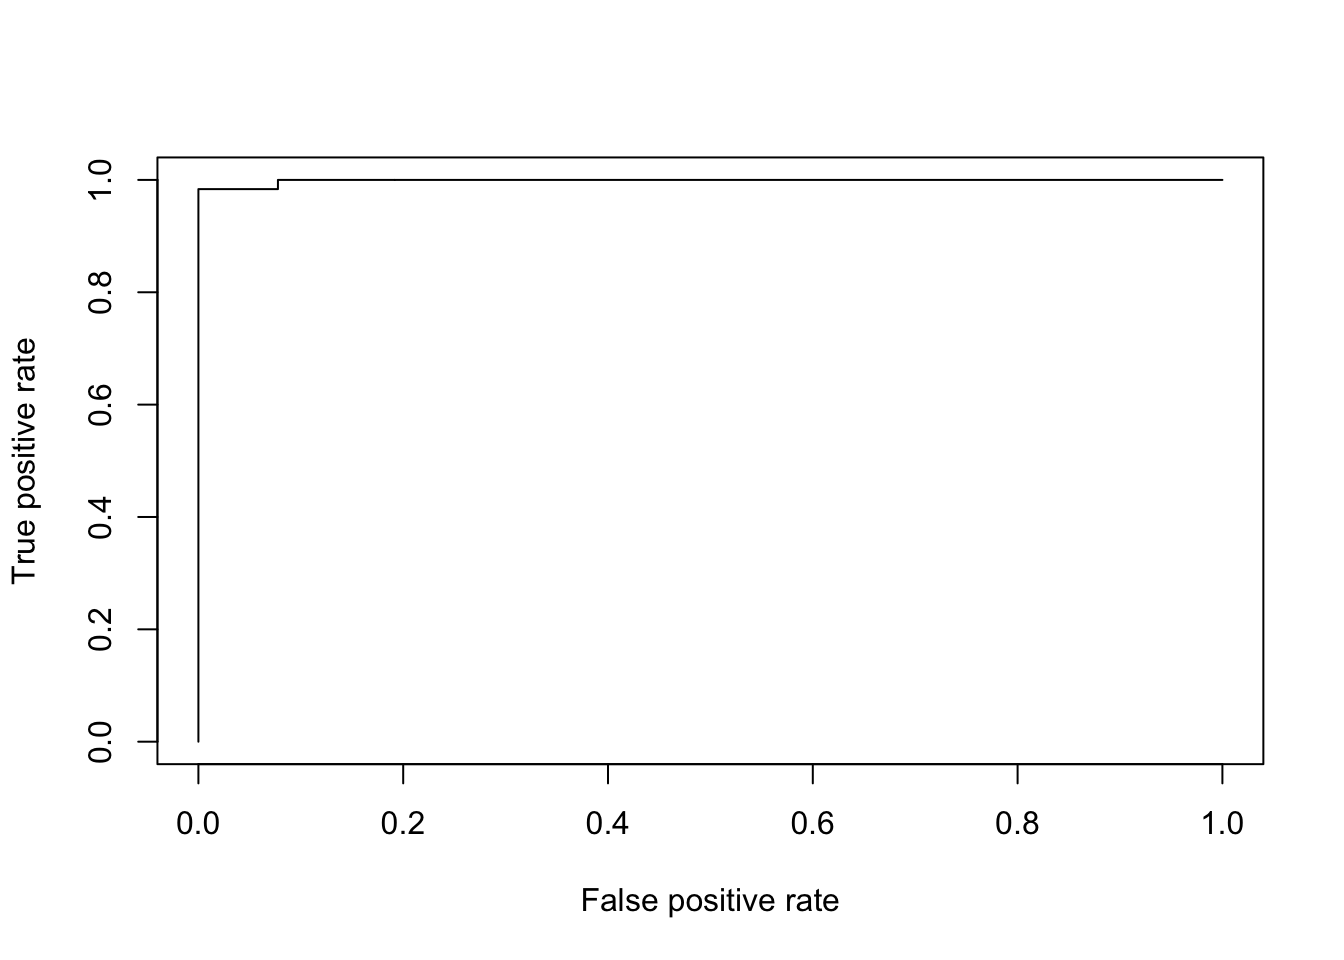
\includegraphics[width=0.45\textwidth]{results/pre-update/memleak/boosting-roc}
  }
  \caption[Pre-Update, Memory Leak Boosting Performance]{Test data performance
  of the boosting prediction method on failure data obtained by consuming all
  available memory until target application fails.}
  \label{fig:memLeakPreUpdateBoostingPerf}
\end{figure*}
}

% Post-Update (old model)
\newcommand{\figMemLeakPostUpdateSameBoostedModel}{\begin{figure*}
  \centering
  \subfigure[Precision/Recall Curve.]{
    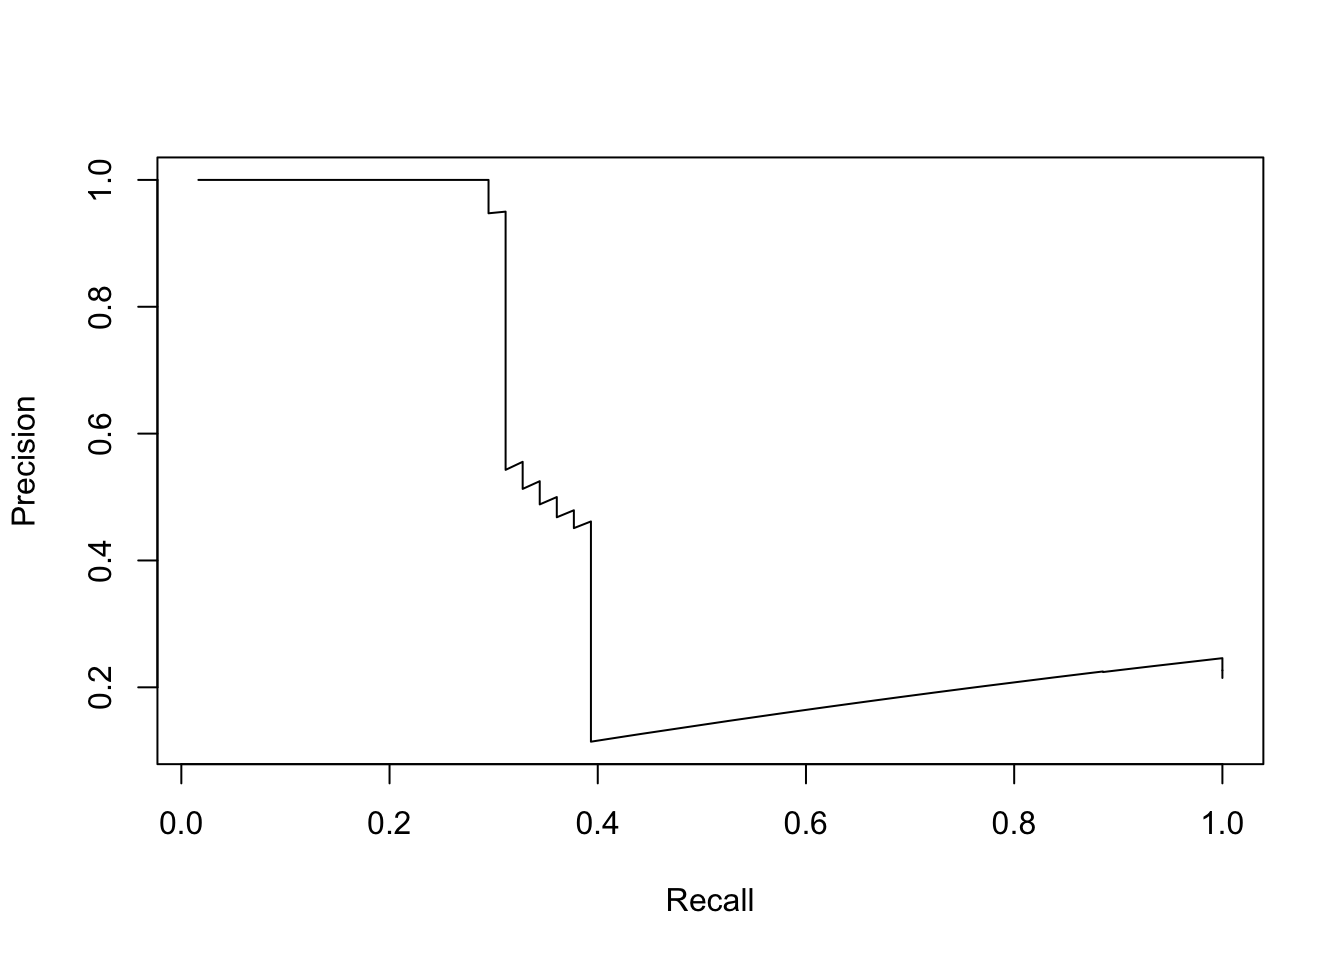
\includegraphics[width=0.45\textwidth]{results/post-update/memleak/boost-samemodel-prc}
  }
  \subfigure[\ac{ROC} Curve (\ac{AUC} = 0.4854).]{
    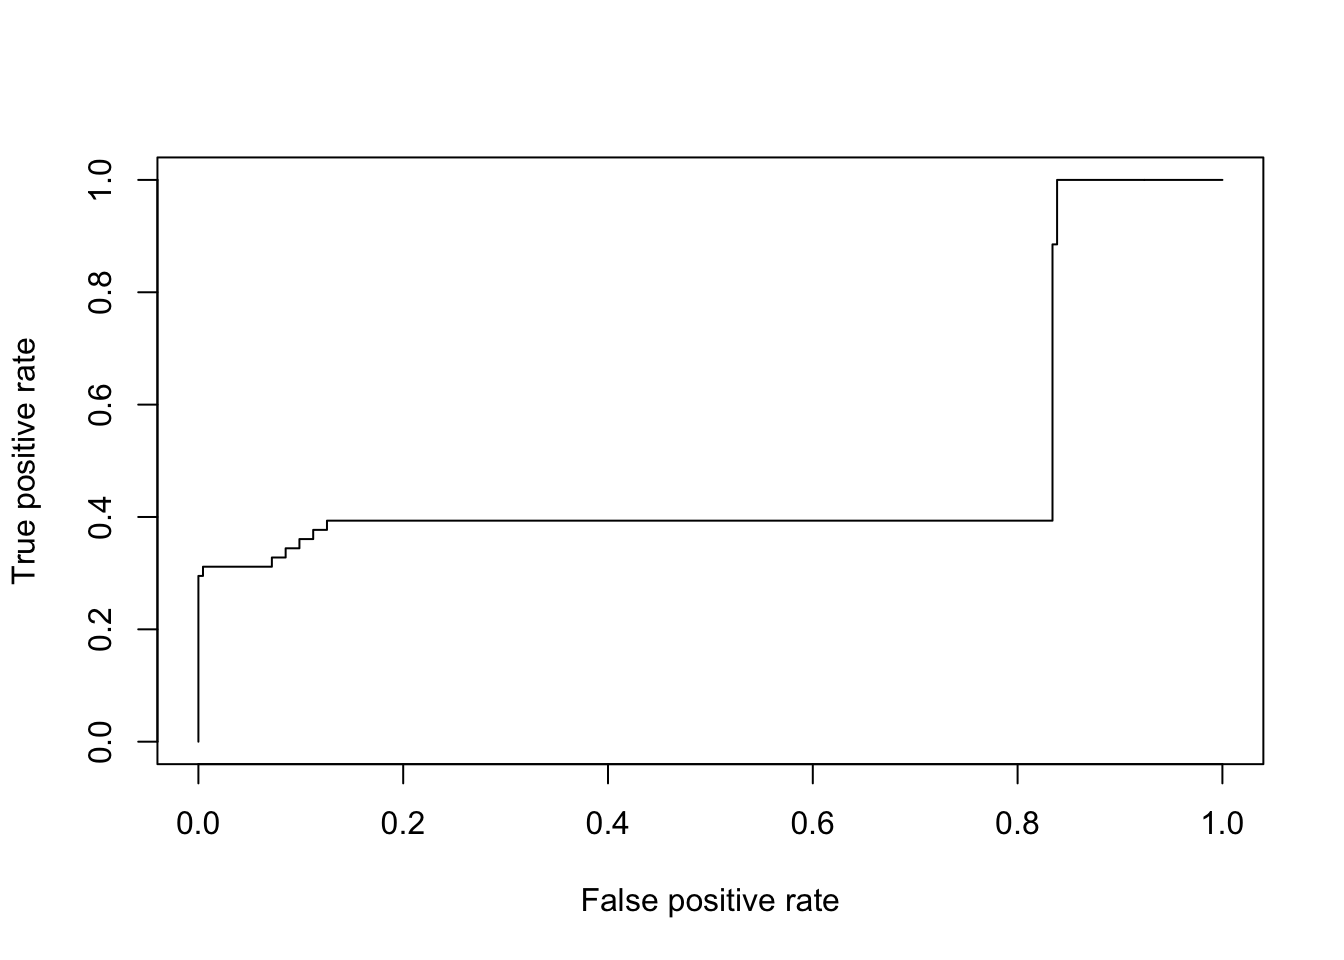
\includegraphics[width=0.45\textwidth]{results/post-update/memleak/boost-samemodel-roc}
  }
  \caption[Post-Update, Memory Leak Using Old Model Performance]{Performance of
  the boosting prediction method trained on failure data created before the
  software update obtained by consuming all available memory until target
  application fails.}
  \label{fig:memLeakPostUpdateSameBoostedModel}
\end{figure*}
}

% Post-Update New Model
\newcommand{\figMemLeakPostUpdateBoostingPerf}{\begin{figure*}
  \centering
  \subfigure[Precision/Recall Curve.]{
    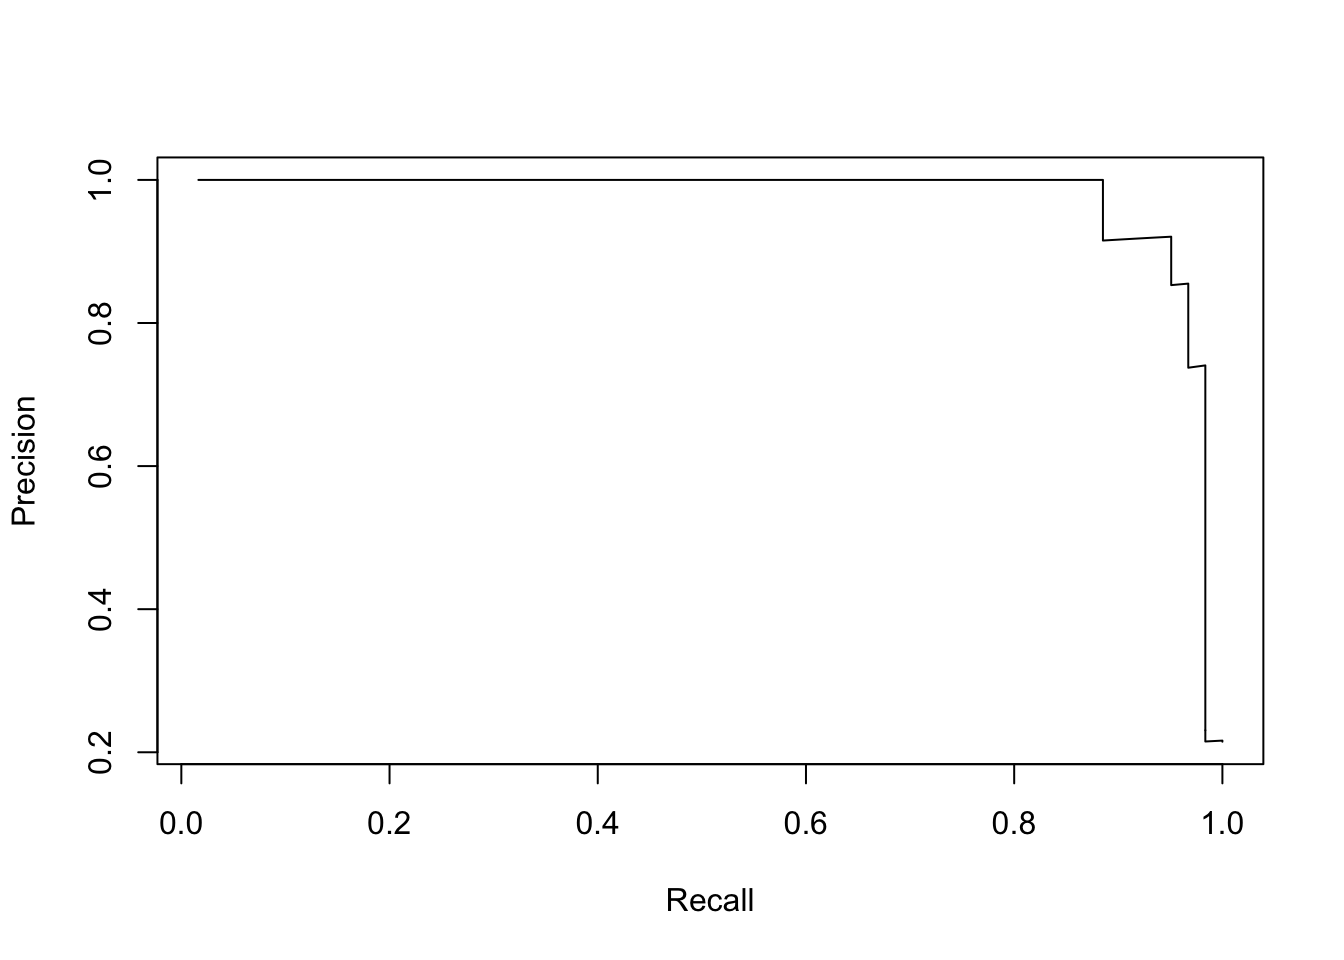
\includegraphics[width=0.45\textwidth]{results/post-update/memleak/boost-prc}
  }
  \subfigure[\ac{ROC} Curve (\ac{AUC} = 0.9801).]{
    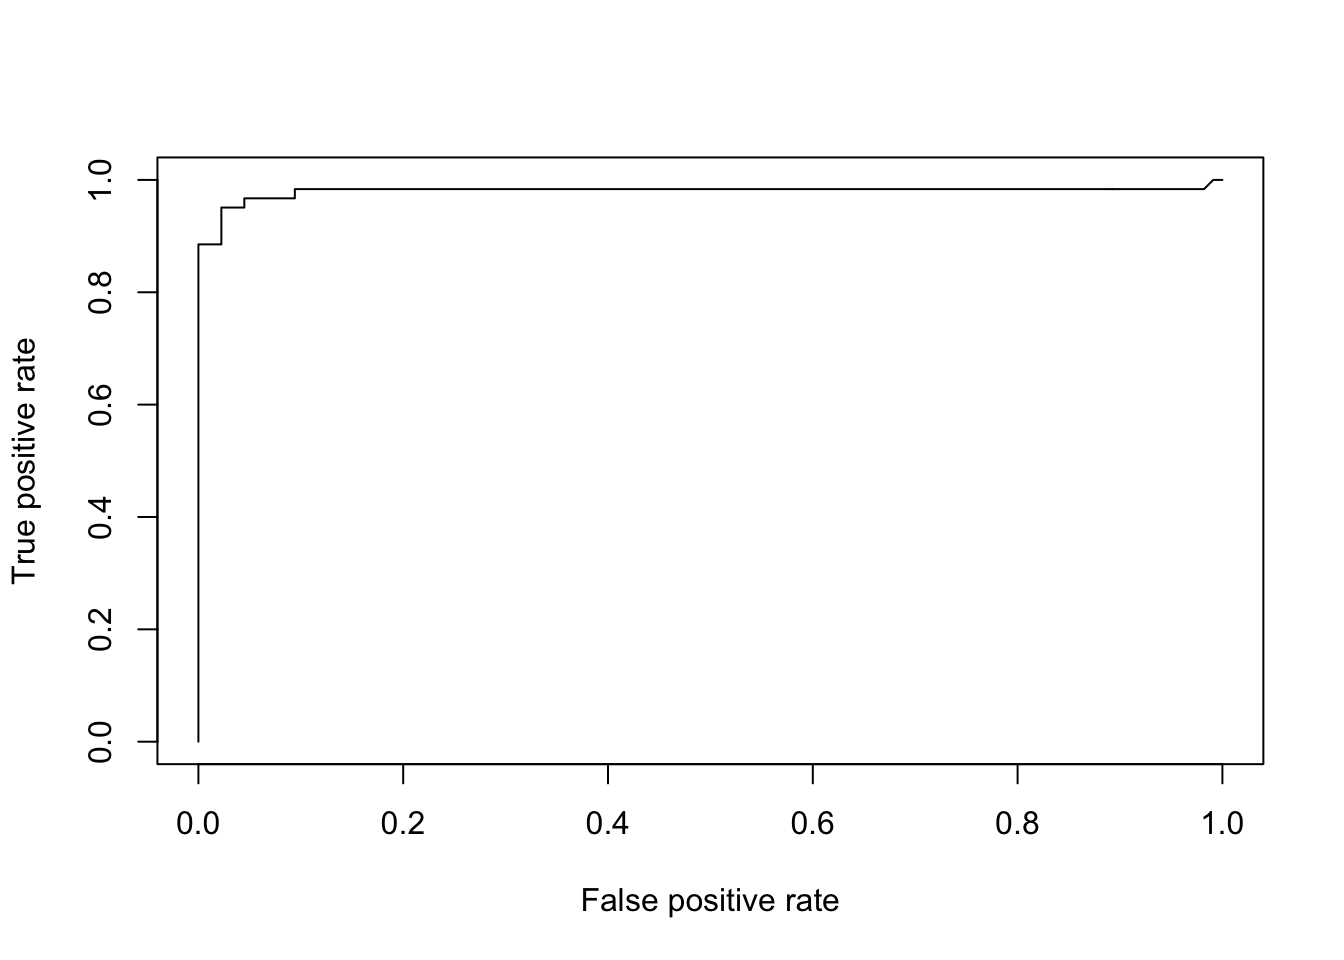
\includegraphics[width=0.45\textwidth]{results/post-update/memleak/boost-roc}
  }
  \caption[Post-Update, Memory Leak Using New Model Performance]{Performance of
  the boosting prediction method trained on failure data created after the
  software update obtained by consuming all available memory until target
  application fails.}
  \label{fig:memLeakPostUpdateBoostingPerf}
\end{figure*}
}

\newcommand{\figDPLGConceptDiagram}[1]{\begin{figure}
  \centering 
  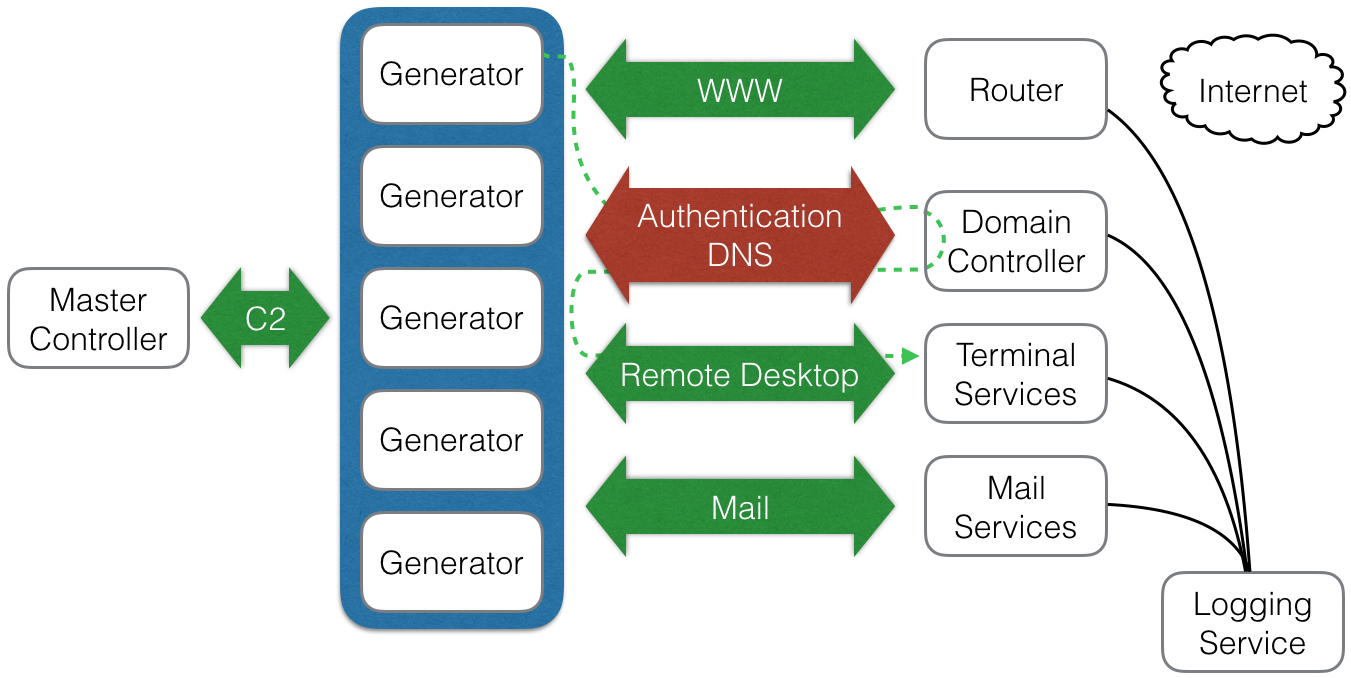
\includegraphics[width=#1]{DPLG/dplgConceptDiagram}
  \caption[Concept Diagram]{How each type of traffic that is generated is
  routed.  Log events are offloaded to logging service for further analysis.}
  \label{fig:conceptDiagram} 
  \end{figure}
}

\newcommand{\figDPLGAllModsClientMetrics}[1]{\begin{figure}
  \centering
  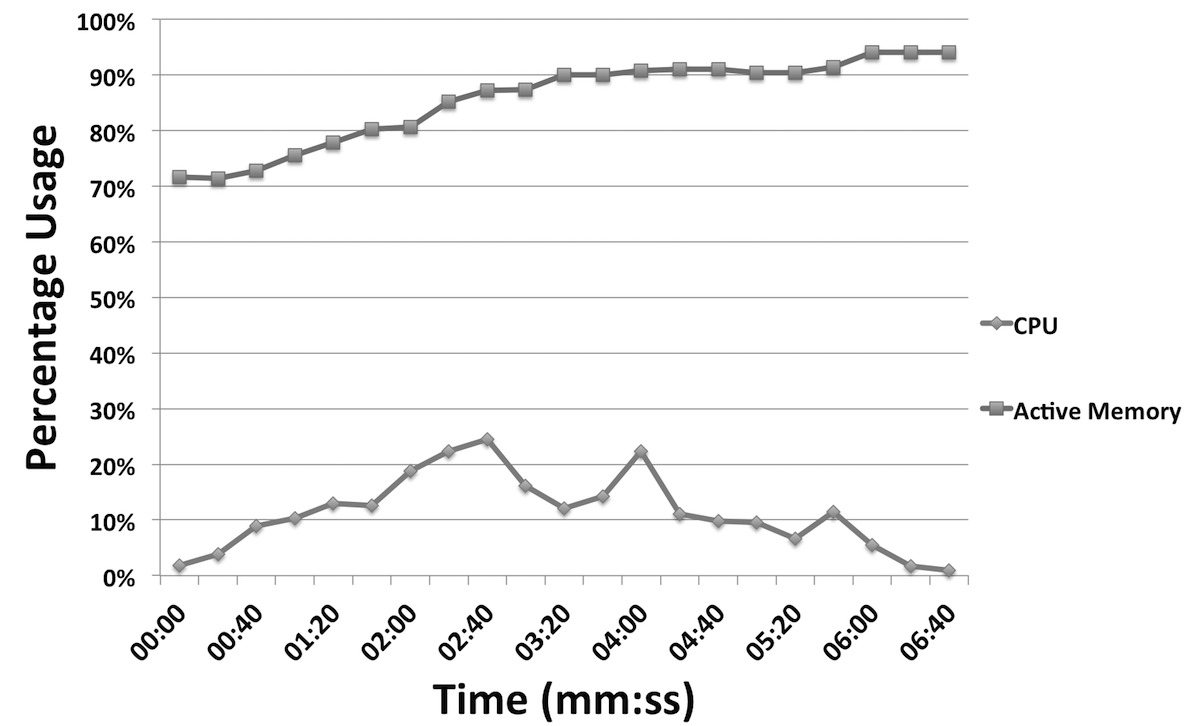
\includegraphics[width=#1]{DPLG/allModsClientMetrics}
  \caption[Test 2:  Client Metrics]{Client CPU and memory utilization during
  the second test.} \label{fig:allModsClientMetrics}
  \end{figure}
}


\newcommand{\tabFaults}{
\begin{table}[htbp]
  \centering
  \caption{Table of Faults Injected~\cite{gswfit}.}\label{tab:faults}
\begin{tabular}{ | c | l | c | } 
\hline
	\textbf{Type}  & \textbf{Description}  & \textbf{ODC Classes}  \\ \hline \hline
	MIFS  & Missing "If (cond) \{ statement(s) \}"  & Algorithm  \\ \hline
	MFC  & Missing function call  & Algorithm  \\ \hline
	MLAC  & Missing "AND EXPR" in expression used as branch & Checking  \\ \hline
	MLPC  & Missing small and localized part of the algorithm  & Algorithm  \\ \hline
	WVAV  & Wrong value assigned to a value  & Assignment  \\ \hline
	MVI  & Missing variable initialization  & Assignment  \\ \hline
	MVAV  & Missing variable assignment using a value  & Assignment  \\ \hline
	WPFV  & Wrong variable used in parameter of function call  & Interface  \\ \hline
\end{tabular}
\end{table}
}

\newcommand{\tabTranslationThirtyTwo}{
\begin{table}[htbp]
  \centering
  \caption{Funtion Entry/Exit Patterns
  (IA32)~\cite{gswfit}.}\label{tab:translationThirtyTwo}
\begin{tabular}{ | l | l | l | l | }
\hline
	\multicolumn{2}{|c|}{\textbf{Module Entry Point}}& 
  \multicolumn{2}{c|}{\textbf{Module Exit Point}} \\ \hline

	\textbf{Instruction Sequence} & \textbf{Explanation} &
  \textbf{Instruction Sequence} & \textbf{Explanation} \\ \hline \hline

	push ebp & stack frame & move esp,ebp & stack frame \\ \hline
	mov ebp, esp & setup & pop ebp & cleanup \\ \hline
	sub esp, \emph{immed} &  & ret &  \\ \hline
\end{tabular}
\end{table}
}

\newcommand{\tabTranslationSixtyFour}{
\begin{table}[htbp]
  \centering
  \caption{Funtion Entry/Exit Patterns
  (x86-64)~\cite{gswfit}.}\label{tab:translationSixtyFour}
\begin{tabular}{ | l | l | l | l | }
\hline
	\multicolumn{2}{|c|}{\textbf{Module Entry Point}}& 
  \multicolumn{2}{c|}{\textbf{Module Exit Point}} \\ \hline

	\textbf{Instruction Sequence} & \textbf{Explanation} & 
  \textbf{Instruction Sequence} & \textbf{Explanation} \\ \hline \hline

	push rbp & stack frame & add rsp, \emph{immed} & stack frame \\ \hline
	sub rsp, \emph{immed} &  & pop rbp & cleanup \\ \hline
	mov rbp, rdx & setup & ret &  \\ \hline
\end{tabular}
\end{table}
}

\newcommand{\tabHypervisorOne}{
\begin{table}[htbp]
  \centering
  \caption{Hypervisor 1 Configuration (Sandbox/Target).} \label{tab:hyp1}
  \begin{tabular}{ | c | l | l | c | l |}
    \hline
    Qty. & Role   & Operating System    & CPU / Mem. \\ \hline\hline
    1    & DC     & Win. Server 2008 R2 & 2 / 2 GB   \\ \hline
    5    & Client & Win. 7              & 1 / 512 MB \\ 
    \hline
  \end{tabular}
\end{table}
}


\newcommand{\tabHypervisorTwo}{
\begin{table}[htbp]
  \centering
  \caption{Hypervisor 2 Configuration (Controller).} \label{tab:hyp2}
  \begin{tabular}{ | c | l | l | c | l |}
    \hline
    Qty. & Role & Operating System    & CPU / Mem. \\ \hline\hline
    1    & RDP  & Win. Server 2008 R2 & 1 / 4 GB   \\ \hline
    1    & Log  & Ubuntu 14.04 LTS    & 1 / 1 GB   \\ 
    \hline
  \end{tabular}
\end{table}
}

\newcommand{\tabMessage}{
\begin{table}[!ht] \centering
  \caption{Typical authentication message sent as keys that correspond to the
  values as designated in the \emph{Snare} protocol for MSWinEventLog used by
  the SolarWinds syslog agent.} \label{tab:message}
  \begin{tabular}{ | l | l | }
    \hline
      Key                 & Value                               \\ \hline\hline
      HostName            & dc.afnet.com                        \\ \hline
      Criticality         & 5                                   \\ \hline
      EventLogSource      & Security                            \\ \hline
      Counter             & 3                                   \\ \hline
      SubmitTime          & Sun May 08 14:31:50 2016            \\ \hline
      EventID             & 4672                                \\ \hline
      SourceName          & Microsoft-Windows-Security-Auditing \\ \hline
      UserName            & N/A                                 \\ \hline
      SIDType             & Audit Success                       \\ \hline
      EventLogType        & dc.afnet.com                        \\ \hline
      ComputerName        & 12548                               \\ \hline
      CategoryString      & Special privileges assigned to\dots \\ \hline
      ExtendedDataString  & Security ID:  S-1-5-21-2379403\dots \\ 
    \hline
  \end{tabular}
\end{table}
}

\newcommand{\tabSlidingWindow}{
\begin{table}[!ht] \centering
  \caption{Sample time window after message translation.} \label{tab:window}
  \begin{tabular}{ | l | l | }
    \hline
      Key                         & Value \\ \hline\hline
      FailureWindow               & 0     \\ \hline
      NumObservations             & 2     \\ \hline
      Criticality: 6              & 2     \\ \hline
      Criticality: 2              & 0     \\ \hline
      Criticality: 4              & 0     \\ \hline
      EventLogSource: Application & 1     \\ \hline
      EventLogSource: System      & 1     \\ 
    \hline
  \end{tabular}
\end{table}
}

\newcommand{\tabMemLeakPreUpdateSVMStats}{
\begin{table}[!t] \centering
  \caption[Pre-Update, Memory Leak, SVM Statistics]{Classification statistics
  on test data created before software updates.}
  \label{tab:memLeakPreUpdateSVMStats}
  \begin{tabular}{ | l | l | }
    \hline
      Statistic           & Value  \\ \hline\hline
      True Positive Rate  & 0.8525 \\ \hline
      False Positive Rate & 0.0098 \\ \hline
      Accuracy            & 0.9777 \\ \hline
      Precision           & 0.8966 \\ \hline
      Recall              & 0.8525 \\ \hline
      F-Measure           & 0.8739 \\
    \hline
  \end{tabular}
\end{table}
}
%%%%%%%%%%%%%%%%%%%%%%%%%%%%%%%%%%%%%%%%%%%%%%%%%%%%%%%%%%%%%%%%%%%%%%%%%%%%%%%
%%%%   SVM   %%%%
% Pre-Update
\newcommand{\tabMemLeakPreUpdateSVMConfusionMatrix}{
  \begin{table}[!ht]
    \centering
    \caption[Pre-Update, Memory Leak, SVM Confusion Matrix]{Confusion matrix on
    test data created before software updates on threshold with highest
    F-Measure (0.8739) using SVM.}
    \label{tab:memLeakPreUpdateSVMConfusionMatrix}
    \begin{tabular}{llll}
                                                               &                                       & \multicolumn{2}{c}{\textbf{Actual}}                                        \\ \cline{3-4} 
                                                               & \multicolumn{1}{l|}{}                 & \multicolumn{1}{l|}{\textbf{Fail}} & \multicolumn{1}{l|}{\textbf{No-Fail}} \\ \cline{2-4} 
      \multicolumn{1}{c|}{\multirow{2}{*}{\textbf{Predicted}}} & \multicolumn{1}{l|}{\textbf{Fail}}    & \multicolumn{1}{l|}{52}            & \multicolumn{1}{l|}{6}                \\ \cline{2-4} 
      \multicolumn{1}{c|}{}                                    & \multicolumn{1}{l|}{\textbf{No-Fail}} & \multicolumn{1}{l|}{9}             & \multicolumn{1}{l|}{607}              \\ \cline{2-4} 
    \end{tabular}
  \end{table}
}

% Post-Update (old model)

% Post-Update New Model

%%%%   BOOSTING   %%%%
% Pre-Update
\newcommand{\tabMemLeakPreUpdateBoostingConfusionMatrix}{
  \begin{table}[!ht]
    \centering
    \caption[Pre-Update, Memory Leak, Boosting Confusion Matrix]{Confusion
    matrix on test data created before software updates on threshold with
    highest F-Measure (0.9917) using boosting.}
    \label{tab:memLeakPreUpdateBoostingConfusionMatrix}
    \begin{tabular}{llll}
                                                               &                                       & \multicolumn{2}{c}{\textbf{Actual}}                                        \\ \cline{3-4} 
                                                               & \multicolumn{1}{l|}{}                 & \multicolumn{1}{l|}{\textbf{Fail}} & \multicolumn{1}{l|}{\textbf{No-Fail}} \\ \cline{2-4} 
      \multicolumn{1}{c|}{\multirow{2}{*}{\textbf{Predicted}}} & \multicolumn{1}{l|}{\textbf{Fail}}    & \multicolumn{1}{l|}{60}            & \multicolumn{1}{l|}{0}                \\ \cline{2-4} 
      \multicolumn{1}{c|}{}                                    & \multicolumn{1}{l|}{\textbf{No-Fail}} & \multicolumn{1}{l|}{1}             & \multicolumn{1}{l|}{412}              \\ \cline{2-4} 
    \end{tabular}
  \end{table}
}

% Post-Update (old model)
\newcommand{\tabMemLeakPostUpdateBoostingSameModelConfusionMatrix}{
  \begin{table}[!ht]
    \centering
    \caption[Post-Update, Memory Leak, Same Model, Confusion
    Matrix]{Post-update failure data confusion matrix on threshold with highest
    F-Measure (0.4691) using model trained on failure data generated before
    software update.}
    \label{tab:memLeakPostUpdateBoostingSameModelConfusionMatrix}
    \begin{tabular}{llll}
                                                               &                                       & \multicolumn{2}{c}{\textbf{Actual}}                                        \\ \cline{3-4} 
                                                               & \multicolumn{1}{l|}{}                 & \multicolumn{1}{l|}{\textbf{Fail}} & \multicolumn{1}{l|}{\textbf{No-Fail}} \\ \cline{2-4} 
      \multicolumn{1}{c|}{\multirow{2}{*}{\textbf{Predicted}}} & \multicolumn{1}{l|}{\textbf{Fail}}    & \multicolumn{1}{l|}{19}            & \multicolumn{1}{l|}{1}                \\ \cline{2-4} 
      \multicolumn{1}{c|}{}                                    & \multicolumn{1}{l|}{\textbf{No-Fail}} & \multicolumn{1}{l|}{42}            & \multicolumn{1}{l|}{222}              \\ \cline{2-4} 
    \end{tabular}
  \end{table}
}

% Post-Update New Model
\newcommand{\tabMemLeakPostUpdateBoostingConfusionMatrix}{
  \begin{table}[!ht]
    \centering
    \caption[Post-Update, Memory Leak, New Model, Confusion
    Matrix]{Post-update failure data confusion matrix on threshold with highest
    F-Measure (0.9355) using model trained on failure data generated after
    software update.}
    \label{tab:memLeakPostUpdateBoostingConfusionMatrix}
    \begin{tabular}{llll}
                                                               &                                       & \multicolumn{2}{c}{\textbf{Actual}}                                        \\ \cline{3-4} 
                                                               & \multicolumn{1}{l|}{}                 & \multicolumn{1}{l|}{\textbf{Fail}} & \multicolumn{1}{l|}{\textbf{No-Fail}} \\ \cline{2-4} 
      \multicolumn{1}{c|}{\multirow{2}{*}{\textbf{Predicted}}} & \multicolumn{1}{l|}{\textbf{Fail}}    & \multicolumn{1}{l|}{58}            & \multicolumn{1}{l|}{5}                \\ \cline{2-4} 
      \multicolumn{1}{c|}{}                                    & \multicolumn{1}{l|}{\textbf{No-Fail}} & \multicolumn{1}{l|}{3}             & \multicolumn{1}{l|}{218}              \\ \cline{2-4} 
    \end{tabular}
  \end{table}
}

%%%%%%%%%%%%%%%%%%%%%%%%%%%%%%%%%%%%%%%%%%%%%%%%%%%%%%%%%%%%%%%%%%%%%%%%%%%%%%%
\newcommand{\tabModelSelection}{
\begin{table*}[!t]
  \centering
  \caption{Cross-validation runs on training data for model selection and
  resulting classification accuracy.}
  \label{tab:model:selection}
  \begin{tabular}{cllllllllllll}
    \multicolumn{1}{l}{}                       & \multicolumn{12}{c}{{\ul \textbf{Amount of Training Data}}}                                                                                                                                                                                         \\ \cline{2-13} 
    \multicolumn{1}{l|}{{\ul \textbf{Window}}} & \multicolumn{4}{c}{One Failure}                                             & \multicolumn{4}{c}{Two Failures}                                                & \multicolumn{4}{c|}{Four Failures}                                              \\ \cline{2-13} 
    \multicolumn{1}{c|}{\multirow{2}{*}{30s}}  & \textbf{Linear:}  & 0.0557 & \textbf{Poly:}   & \multicolumn{1}{l|}{0.0523} & \textbf{Linear:}  & 0.0756 & \textbf{Poly:}   & \multicolumn{1}{l|}{0.0659} & \textbf{Linear:}  & 0.0733 & \textbf{Poly:}   & \multicolumn{1}{l|}{0.0547} \\
    \multicolumn{1}{c|}{}                      & \textbf{Sigmoid:} & 0.0626 & \textbf{Radial:} & \multicolumn{1}{l|}{0.0459} & \textbf{Sigmoid:} & 0.0591 & \textbf{Radial:} & \multicolumn{1}{l|}{0.0438} & \textbf{Sigmoid:} & 0.0794 & \textbf{Radial:} & \multicolumn{1}{l|}{0.0542} \\ \cline{2-13} 
    \multicolumn{1}{c|}{\multirow{2}{*}{60s}}  & \textbf{Linear:}  & 0.0628 & \textbf{Poly:}   & \multicolumn{1}{l|}{0.0662} & \textbf{Linear:}  & 0.0779 & \textbf{Poly:}   & \multicolumn{1}{l|}{0.064}  & \textbf{Linear:}  & 0.0791 & \textbf{Poly:}   & \multicolumn{1}{l|}{0.0779} \\
    \multicolumn{1}{c|}{}                      & \textbf{Sigmoid:} & 0.1084 & \textbf{Radial:} & \multicolumn{1}{l|}{0.0487} & \textbf{Sigmoid:} & 0.1328 & \textbf{Radial:} & \multicolumn{1}{l|}{0.071}  & \textbf{Sigmoid:} & 0.2159 & \textbf{Radial:} & \multicolumn{1}{l|}{0.0797} \\ \cline{2-13} 
    \multicolumn{1}{c|}{\multirow{2}{*}{90s}}  & \textbf{Linear:}  & 0.1272 & \textbf{Poly:}   & \multicolumn{1}{l|}{0.0897} & \textbf{Linear:}  & 0.1131 & \textbf{Poly:}   & \multicolumn{1}{l|}{0.0732} & \textbf{Linear:}  & 0.0826 & \textbf{Poly:}   & \multicolumn{1}{l|}{0.0543} \\
    \multicolumn{1}{c|}{}                      & \textbf{Sigmoid:} & 0.1792 & \textbf{Radial:} & \multicolumn{1}{l|}{0.0779} & \textbf{Sigmoid:} & 0.2684 & \textbf{Radial:} & \multicolumn{1}{l|}{0.0757} & \textbf{Sigmoid:} & 0.2404 & \textbf{Radial:} & \multicolumn{1}{l|}{0.0552} \\ \cline{2-13} 
    \multicolumn{1}{c|}{\multirow{2}{*}{120s}} & \textbf{Linear:}  & 0.132  & \textbf{Poly:}   & \multicolumn{1}{l|}{0.104}  & \textbf{Linear:}  & 0.1452 & \textbf{Poly:}   & \multicolumn{1}{l|}{0.0785} & \textbf{Linear:}  & 0.0998 & \textbf{Poly:}   & \multicolumn{1}{l|}{0.0705} \\
    \multicolumn{1}{c|}{}                      & \textbf{Sigmoid:} & 0.204  & \textbf{Radial:} & \multicolumn{1}{l|}{0.104}  & \textbf{Sigmoid:} & 0.2864 & \textbf{Radial:} & \multicolumn{1}{l|}{0.0585} & \textbf{Sigmoid:} & 0.3056 & \textbf{Radial:} & \multicolumn{1}{l|}{0.0792} \\ \cline{2-13} 
  \end{tabular}
\end{table*}
}

% define custom commands
\newcommand{\regmark}{\raisebox{5pt}{\tiny \circledR}\xspace}
\newcommand{\matlab}{\textsc{Matlab}\regmark}
\newcommand{\trademark}{\raisebox{5pt}{\tiny TM}\xspace}
\newcommand{\mca}{\texttt{Mathematica}\regmark}
\newcommand{\Latex}{\LaTeX\xspace}

% Create a new theorem style called a Corollary.
% If you don't have any, then just comment this out.
%\theoremstyle{plain} % Default
\newtheorem{cor}{Corollary}[chapter]

%Custom Commands for Student

\newcommand{\primerAddress}{{L:$\backslash$Courses$\backslash$PHYS$\backslash$LaTeX}\xspace}

\begin{document}

\frontmatter
	\flyleaf                        
	\disclaimerpage                 
	\titlepageAFIT                      
	\committeepage  
	A framework for automating the training and deployment of failure prediction
algorithms has recently been introduced.  Unfortunately, the framework was only
tested on a single deprecated operating system.  In order to generalize the
approach a few key functions must be performed, one of which being realistic
workload generation.  Unfortunately, a workload generator capable of generating
sufficient workload has not been developed for a Microsoft Windows active
directory environment.  In this paper we introduce and detail a tool that we
have developed to make the implementation of this new framework possible on a
modern Microsoft operating system, we present data generated by our tool to
demonstrate its efficacy, and finish with several extensions and applications
for our tool.

	\begin{acknowledgements}

I would like to thank...


\end{acknowledgements}

	\tableofcontents
	\listoffigures
	\listoftables
\mainmatter

%%%%%%%%%%%%%%%%%%%%%%%%%%%%%%%%%%%%%%%%%%%%%%%%%%%%%%%%%%%%%%%%%%%%%%%%%%%%%%%
%%%%                                CHAPTER 1                              %%%%
%%%%%%%%%%%%%%%%%%%%%%%%%%%%%%%%%%%%%%%%%%%%%%%%%%%%%%%%%%%%%%%%%%%%%%%%%%%%%%%
\chapter{Introduction}
As we become more dependent upon computers and they permeate their way into our
daily lives, we need to consider the risks associated.  Computer systems are
literally all around us.  Some of these computer systems play insignificant
roles in our lives while others may be responsible for sustaining our lives.
Unfortunately, the software that controls these systems is written by humans
and consequently subject to human error.  As a result, these systems are prone
to failure which in many cases may not be a big deal, but in others, could have
severe consequences.  Every day, critical infrastructure and Air Force missions
systems depend on the reliability of computer systems.  As a result, being able
to predict pending failue in computer systems can offer tremendous and
potentially life-saving applications in todays technologically advanced world.
While actually being able to accurately predict failure has unfortunately not
been proven possible, there has been an enormous amount of time and energy
spent over the past several decades attempting to make educated predictions
about the failure of machines through the use of sophisticated machine learning
algorithms.  Unfortunately, much of this work has gone unused.  

There a number of ways to reduce the number of errors produced by a piece of
software, but the software development life-cycle is shrinking and less time
and effort are being devoted to reducing errors before deployment.  This leaves
real-time error prevention or handling.  In recent years, it seems many of the
cloud based computing companies have attempted to solve problems caused by
machine failure by making all of their services massively redundant.  As
hardware becomes more affordable, this is an effective approach in many ways,
but ultimately is still not cost efficient.  In some cases, funds may not be
available to acheive this sort of redundancy.  Consequently, this research
focuses on a small piece of the general field of reliable computing: online
failure prediction (OFP).  OFP is the act of attempting to predict when
failures are likely so that they can be avoided.  A great deal of work has been
done in this field which we outline in Chapter~\ref{chapter2}, but much of it
has gone unimplemented due to the complex and manual task of training a
prediction model.  If the underlying system changes at all the efficacy of a
prediction model can be drastically reduced if not rendered completely useless
until it is retrained.  Furthermore, training requires access to labelled
training data.  Since failure is such a rare event, access to this type of
training data may not be possible.  

Irrera et al.~\cite{irrera2015} presented a potential solution in 2015 to
automate the process of dynamically generating failure data and using it to
train a predictor after an underlying system change.  They defined a framework
for implementing this process and called it the Adaptive Failure Prediction
(AFP) Framework.  This research explores an implementation of that framework.
More specifically, we present our results after implementing the AFP using a
Microsoft Windows Server domain controller.  We then apply successive software
updates until the model we have selected becomes useless and allow the
framework to re-train our predictor.

\section{Problem Statement}
Predicting and alerting on impending network service failures currently uses
thresholds and rules on discrete items in enterprise system logs.  For example,
if the central processing unit (CPU) and memory usage on a device exceeds 90\%,
then an alert may be issued.  This approach works, but only for certain types
of failures and in order to minimize the false positives, it only makes
recommendations minutes before a failure, or when the system is in an already
degraded performance mode.  To maintain network resilience, the operational
organizations responsible for communications support desperately need some
means of gaining lead-time before a service failure occurs.  

Preceding a service failure event, multiple indicators spread disparate
sources, perhaps over a long period of time, may appear in system logs.  The
log entries of interest are also quite rare compared with normal operations.
Because of these constraints, identifying failure indicators can be nearly
impossible for humans to perform.  Further, in most cases, restoring service is
more important than identifying the indicators that may or may not have
existed.  

Failure prediction can be approached in many ways. Arguably the simplest
approach is to use everyday statistical analysis to, for example, determine the
mean time between failures of specific components. The analysis of all
components making up a system can be aggregated to make predictions about that
system using a set of statistics-based or business-relevant rules.
Unfortunately, the complexity of modern architectures has outpaced such
off-line statistical-based analysis, which has driven the advancement of OFP.
OFP differs from other means of failure prediction in that it focuses on
classifying the current running state of a machine as either failure prone or
not, or in such a way that it describes the confidence in how failure prone a
system is at present~\cite{salfnerSurvey}.

Unfortunately, in recent years much of the work in OFP has gone unused due to
the dramatic decrease in cost and complexity involved in building
hardware-based redundant systems.  Furthermore, in most cases OFP implements
machine learning algorithms that require manual re-training after underlying
system changes.  More troubling is that these system changes are becoming more
frequent as the software development life cycle moves toward a more continuous
integration model.  To help solve these challenges, the framework presented
in~\cite{irrera2015} uses simulated faults to automatically re-train a
prediction algorithm to make implementing OFP approaches easier.  We propose to
expand the work in~\cite{irrera2015} to capture developments since its writing
and generalize it so it works for a broader class of devices.

\section{Impact of Research}
Every day, many of the Air Force's critical missions depend on our computer
infrastructure.  An essential piece of this infrastructure is the
authentication mechanisms that protect our sensitive information.
Unfortunately, the software at the core of this infrastructure is written and
maintained by humans and thus susceptible human error.  This research will
enable the Air Force and many others that use the Microsoft Enterprise
Infrastructure to accurately predict pending service outages thereby providing
lead-time in order to avoid those outages.  The result is cost savings in
personnel, equipment, but isn't limited to cost savings.  It is difficult to
quantify the risk of mission failure due to network service outage.

\section{Assumptions and Limitations}
As previously stated, it has not been proven possible to accurately predict
future events without a priori knowledge.  As a result, this research depends
on the fact that there are indicators of failure present and available to us
with enough lead-time to accurately make decisions and take mitigation action
should failure be predicted based on these indicators.  This research presents
a method of predicting failure, but this method is completely useless at
predicting \emph{act of God} events.  Further, this method is capable of
predicting failure based on software failures and cannot provide any useful
information about malicious attacks against the target software.

\section{Expected Results of Research}
Because a prediction method is not presently deployed on any Air Force network,
any level of dependable prediction will be better than what is currently
available.  This research will attempt to show that after an underlying system
change, this method of predicting failure will be capable of automatically
training a more effective prediction algorithm so that this technique can be
implemented on an Air Force network with little to no impact on manpower.
Consequently, we expect that this research will inform decision makers and
allow them to implement this technique in a production environment.

Specifically, we believe the technique presented in this research could most
effectively be implemented and used by the Cyber Security and Control System
(CSCS) weapon system employed at the 561st and 83d Network Operation Squadrons
(NOS) and their associated detachments to reduce the number of network service
outages, increasing uptime, leading to improved mission effectiveness in both
the support and operational domains.  Further, we believe this technique
general enough to be employed outside of the Air Force to increase mission
effectiveness across the Department of Defense (DOD).  External to the DOD,
this research further generalizes an approach that could be used to help
increase availability of nearly any computer system.


%%%%%%%%%%%%%%%%%%%%%%%%%%%%%%%%%%%%%%%%%%%%%%%%%%%%%%%%%%%%%%%%%%%%%%%%%%%%%%%
%%%%                                CHAPTER 2                              %%%%
%%%%%%%%%%%%%%%%%%%%%%%%%%%%%%%%%%%%%%%%%%%%%%%%%%%%%%%%%%%%%%%%%%%%%%%%%%%%%%%
\chapter{Overview of Online Failure Prediction} \label{chapter2}
This chapter reviews current research regarding online failure prediction and
its many approaches to build a foundation for this research.  Further, a
taxonomy of approaches was developed here~\cite{salfnerSurvey}, this chapter
updates that taxonomy and classifies approaches since its publication using it.

\section{Background} \label{background}
In 2010, Salfner et al. published a survey paper that provides a comprehensive
summary of the state of the art on the topic of OFP~\cite{salfnerSurvey}.  In
addition to the review of the literature up to the point of publication, they
provide a summary of definitions (see Section~\ref{definitions}) and measures
of performance (see Section~\ref{metrics}) commonly used in the community for
couching the OFP discussion.

\subsection{Definitions} \label{definitions}
\subsubsection{Proactive Fault Management:} \label{pfm}
Salfner, et al.~\cite{salfnerSurvey} define proactive fault management (PFM) as
the process by which faults are handled in a proactive way, analogous with
\emph{fault tolerance} and basically consisting of four steps: online failure
prediction, diagnosis, action scheduling, and action execution as shown in
Figure~\ref{fig:proactiveFaultManagement}.
The final three stages of PFM define how much lead time is required to avoid a
failure when predicted during OFP.  \emph{Lead time} is defined as the time
between when failure is predicted and when that failure will occur.  Lead time
is one of the most critical elements of a failure prediction approach.

\figproactiveFaultManagement

OFP is defined as the first step in PFM shown in
Figure~\ref{fig:proactiveFaultManagement}.  OFP is the act of analyzing the
running state of a system in order to predict a failure in that system. Once
failure has been predicted, a fault tolerant system must determine what will
cause the failure.  This stage is called the \emph{diagnosis} stage or
``root-cause analysis'' stage.  During the \emph{diagnosis} stage, the analysis
must be conducted so that a system knows which remediation actions are
possible.  After it is determined what will cause a failure, a fault tolerant
system must schedule a remediation action that is either performed by an
operator or done automatically.  This stage is known as the \emph{action
scheduling} stage and normally takes as input the cost of performing an action,
confidence in prediction, effectiveness/complexity of remedy action and makes a
decision about what action to perform based on that input.  In some cases a
remedy action can be so simple that even if the confidence in the prediction is
low, the action can still be performed with little impact on the overall system
and its users.  A thorough analysis of the trade-off between cost of avoidance
and confidence in prediction and the associated benefits is described
in~\cite{candea2004microreboot}.  Finally, in order to avoid failure, a system
must execute the scheduled remediation action or let an operator know which
actions can be taken in a stage called \emph{action execution}.

\subsubsection{Faults, Errors, Symptoms, and Failures:}
This research uses the definitions from~\cite{avivzienis2004basic} as
interpreted and extended in~\cite{salfnerSurvey} for the following terms:
failure; error (detected versus undetected); fault; and symptom.

\emph{Failure} is an event that occurs when the delivered service deviates from
correct service.  In other words, things can go wrong internally; as long as
the output of a system is what is expected, failure has not occurred.  

An \emph{error} is the part of the total state of the system that may lead to
its subsequent service failure.  \emph{Errors} are characterized as the point
when things go wrong~\cite{salfnerSurvey}.  Fault tolerant systems can handle
errors without necessarily evolving into failure.  There are two kinds of
errors.  First, a \emph{detected error} is an error that is reported to a
logging service.  In other words, if it can be seen in a log then it is a
detected error.  Second, \emph{undetected errors} are errors that have not been
identified by an error detector.  Undetected errors are things like memory
leaks.  The error exists, but as long as there is usable memory, it is not
likely to be reported to a logging service.  Once the system runs out of usable
memory, undetected errors will likely appear in logs and become a detected
errors.  A \emph{fault} is the hypothesized root cause of an error.  Faults can
remain dormant for some time before manifesting themselves and causing an
incorrect system state.  In the memory leak example, the missing \emph{free}
statement in the source code would be the fault.  

A \emph{symptom} is an out-of-norm behavior of a system's parameters caused by
errors, whether detected or undetected.  In the memory leak example, a possible
symptom of the error might be delayed response times due to sluggish
performance of the overall system.

\figfailureFlowDiagram

Figure~\ref{fig:failureFlowDiagram} illustrates how a software fault can evolve
into a failure.  Faults, errors, symptoms, and failures can be further
categorized by how they are detected also shown in
Figure~\ref{fig:failureFlowDiagram}.  Salfner, et al.~\ref{salfnerSurvey}
introduces a taxonomy of OFP approaches and classifies failure prediction
approaches by the stage at which a fault is detected as it evolves into a
failure: auditing, reporting, monitoring, and tracking.  Testing is left out
because it does not help detect faults in an online sense.  

\figonlinePrediction

Figure~\ref{fig:onlinePrediction} demonstrates the timeline associated with
OFP.  The parameters used by the community to define a predictor are as
follows:
\begin{itemize}
	\item{Present Time: $t$}
  \item{Lead Time: $\Delta t_{l}$, is the total time at which a predictor makes
  an assessment about the current state.}
  \item{Data Window: $\Delta t_{d}$, represents the time from which data is
  used for a predictor uses to make its assessment.}
  \item{Minimal Warning Time: $\Delta t_{w}$, is the amount of time required to
  avoid a failure if one is predicted.}
  \item{Prediction Period: $\Delta t_{p}$, is the time for which a prediction
  is valid.  As $\Delta t_{p} \rightarrow \infty$, the accuracy of the
  predictor approaches 100\% because every system will eventually fail.  As
  this happens, the usefulness of a predictor is diminished.}
\end{itemize}

As the above parameters are adjusted, predictors can become more or less
useful.  For example, it is clear that as a predictor looks further into the
future potentially increasing \emph{lead time}, confidence in its prediction is
likely to be reduced.  On the other hand, if \emph{lead time} is too small,
there will likely not be enough time to effectively take remediation action.
In general, OFP approaches seek to find a balance between the parameters,
within an acceptable bound depending on application, to achieve the best
possible performance.

\subsection{Measures of Performance} \label{metrics}
In order to accurately compare OFP approaches, standard measures of performance are used.  A widely accepted set of measures of performance used by the community is presented in~\cite{salfnerSurvey}.  Before we begin the outline of the measures of performance used to evaluate and compare failure prediction approaches, it is important to note that OFP is done based on statistical analysis of known data.  In other words, in order to calculate the following outlined measures of performance, predictors must be evaluated against labeled data sets.  Typically, the labeled data set is divided into three parts:
\begin{enumerate}
\item{Training Set:  A data set that allows a prediction model to establish and optimize its parameters}
\item{Validation Set:  The parameters selected in the training phase are then validated against a separate data set}
\item{Test Set:  The predictor is finally run against a final previously unevaluated data set to assess generalizability}
\end{enumerate}
During the test phase, true positives (negatives) versus false positives (negatives) are determined in order to compute the measures of performance in this section.  The following terms and associated abbreviations are used: \emph{True Positive} (TP) is when failure has been predicted and then actually occurs; \emph{False Positive} (FP) is when failure has been predicted and then does not occur; \emph{True Negative} (TN) is when a state has been accurately classified as non-failure prone; \emph{False Negative} is when a state has been classified as non-failure prone and a failure occurs.

\subsubsection{Precision and Recall:}
Precision and recall are the most popular measures of performance used when presenting and comparing OFP approaches.  The two are related and often times improving precision results in reduced recall.  For example, if a predictor is more accurate with a prediction then that predictor may be less likely to classify a state as failure-prone in an effort to minimize false-positives.

Precision is the number of correctly identified failures over number of all predicted failures.  In other words, it reports, out of the predictions of a failure-prone state that were made, how many were correct.  In general, the higher the precision the better the predictor.  Precision is expressed as:
\[ Precision 
	= \dfrac{TP}{TP + FP} \in [0,1]
\]

Recall is the ratio of correctly predicted failures to the number of true failures.  In other words, it reports, out of the actual failures that occurred, how many the predictor classified as failure-prone.  In conjunction with a higher precision, higher recall is indicative of a better predictor.  Recall is expressed as:
\[ Recall 
	= \dfrac{TP}{TP + FN} \in [0,1]
\]

F-Measure, as defined by~\cite{rijsbergen1979v}, is the harmonic mean of precision and recall and represents a trade-off between the two.  A higher F-Measure reflects a higher quality predictor.  F-Measure is expressed as:
\[ F\mhyphen Measure 
	= \dfrac{2 \cdot Precision \cdot Recall}{Precision + Recall} \in [0,1]
\]

\subsubsection{False Positive Rate and Specificity:}
Precision and recall do not account for true negatives (correctly predicted non-failure-prone situations) which can bias an assessment of a predictor.  The following measures of performance take true negatives into account to help evaluators more accurately assess and compare predictors.

False Positive Rate (FPR) is the number of incorrectly predicted failures over the total number of predicted non-failure-prone states.  A smaller FPR reflects a higher quality predictor.  The False Positive Rate is expressed as:
\[ \mathit{FPR}
	= \dfrac{FP}{FP + TN} \in [0,1]
\]

Specificity the number of times a predictor correctly classified a state as non-failure-prone over all non-failure-prone predictions made.  In general, specificity alone is not very useful since failure is rare.  Specificity is expressed as:
\[ Specificity 
	= \dfrac{TN}{FP + TN} = 1 - False Positive Rate
\]

\subsubsection{Negative Predictive Value (NPV) and Accuracy:}
In some cases, we wish to show that a prediction approach can correctly classify non-failure-prone situations.  The following measures of performance usually can not stand alone due to the nature of failures being rare events.  In other words, a highly ``accurate'' predictor could classify a state 100\% of the time as non-failure-prone and still fail to predict every single true failure.

Negative Predictive Value (NPV) is the number of times a predictor correctly classifies a state as non-failure-prone to the total number all non-failure-prone states during which a prediction was made.  Higher quality predictors have high NPVs.  The NPV is expressed as:
\[ \mathit{NPV}
	= \dfrac{TN}{TN + FN}
\]

Accuracy is the ratio of all correct predictions to the number of predictions made.  Accuracy is expressed as:
\[ Accuracy 
	= \dfrac{TP + TN}{TP + FP + FN + TN}
\]

\subsubsection{Precision/Recall Curve:}
Much like with other predictors, many OFP approaches implement variable thresholds to sacrifice precision for recall or vice versa.  That trade-off is typically visualized using a precision/recall curve as seen in Figure~\ref{fig:precisionRecallCurve}.

\figprecisionRecallCurve

Another popular visualization is the receiver operating characteristic (ROC) curve.  By plotting true positive rate over false positive rate one is able to see the predictors ability to accurately classify a failure.  A sample ROC curve is shown in Figure~\ref{fig:ROC}.

\figROC

The ROC curve relationship can be further illustrated by calculating the area under the curve (AUC).  Predictors are commonly compared using the AUC which is calculated as follows:

$$AUC = \int_{0}^{1} \mathit{tpr}(\mathit{fpr}) \,d\,\mathit{fpr} \in [0,1],$$

\noindent
where $tpr$ = true positive rate (recall), and $fpr$ = false positive rate.  A pure random predictor will result in an AUC of $0.5$ and a perfect predictor a value of~$1$.  The AUC can be thought of as the probability that a predictor will be able to accurately distinguish between a failure-prone state and a non-failure-prone state, over the entire operating range of the predictor.


\section{Approaches to Online Failure Prediction (OFP)} \label{approaches}
\subsection{OFP Taxonomy}
Taxonomies offer natural ways of organizing information and due to the significant body of work surrounding OFP, one was published by Salfner et al. in 2010~\cite{salfnerSurvey} classifying many of the OFP approaches in the literature into four major categories.  As stated in Section~\ref{definitions}, these four major categories are defined by the four techniques used to detect faults in real-time: auditing, monitoring, reporting, and tracking.  In this research, we update the \emph{reporting} category by classifying approaches to OFP published since its inception.  Since this research focusses on real-time \emph{data-driven} device failure prediction approaches, our focus is on the \emph{reporting} category of Salfner's taxonomy.  The \emph{reporting} category organizes failure prediction techniques that attempt to classify a state as failure prone based on reported errors.  Salfner et al. further organize the reporting category into five sub-categories: rule-based systems; co-occurrence; pattern recognition; statistical tests; classifiers and they are defined as follows:

\emph{Rule-Based Systems} attempt to classify a system as being failure-prone or not based a set of conditions met by reported errors.  Since modern systems are far too complex to build a set of conditions manually, these approaches seek to find automated ways of identifying these conditions in training data.  \emph{Co-occurrence} predictors generate failure predictions based on the reported errors that occur either spatially or temporally close together.  \emph{Pattern Recognition} predictors attempt to classify patterns of reported errors as failure prone.  This research focusses on pattern recognition OFP approaches, which can be visualized in Figure~\ref{fig:patternRecognition}.  \emph{Statistical Tests} attempt to classify a system as failure-prone based on statistical analysis of historical data.  For example, if a system is generating a much larger volume of error reports than it typically does, it may be a sign of pending failure.  \emph{Classifiers} assign labels to given sets of error reports in training data and then make failure predictions based on observed labels in real-time data.

\figpatternRecognition

\subsection{Data-Driven Online Failure Prediction}
The survey published by Salfner et al. covered approaches in every sub-category of the \emph{reporting} category.  Since the publication of the survey, we found approaches in two of the subcategories, \emph{pattern recognition} and \emph{classifiers}.  We therefore only cover the approaches in those sub-categories of the reporting category here.  We found some of the approaches published since Salfner's survey to be difficult to classify because they employ aspects of the other sub-categories in the \emph{reporting} category.  More specifically, many of the modern techniques seem to be a blend between the two sub-categories \emph{pattern recognition} and \emph{classifiers}.  We believe these categories have been blended because these approaches seem to follow general human intuition when looking for software failures.  In other words, we have found that cyber operators tend to look for patterns in reported errors and then classify a situation based on those patterns.  We therefore categorize these approaches as \emph{hybrid} approaches.

\subsubsection{Pattern Recognition:}
In 2006, Salfner et al. proposed an approach to predicting failures by learning patterns of similar events using a semi-Markov chain model~\cite{salfner2006}.  The model learned patterns of error reports that led to failure by mapping the reported errors to the states in the Markov chain and predicted the probability of the transition to a failure-prone state.  They tested the model using performance failures of a telecommunication system and reported a precision of 0.8, recall of 0.923, and an F-measure of 0.8571, which drastically outperformed the models to which it was compared.

Given the results, the semi-Markov Chain model is compelling however, it depends on the sequence of reported errors to remain constant in order to be effective.  Today, most software is multi-threaded or distributed so there is no guarantee that the sequence of reported errors will remain constant.  Further, the authors reported that this approach did not scale well as the complexity of the reported errors grew.

In 2007, Salfner et al. extended their previous work in~\cite{salfner2006} using semi-Markov models~\cite{salfner2007}.  They generalized the Hidden Semi-Markov process for a continuous-time model and called it the ``Generalized Hidden Semi-Markov Model (GHSMM)''  By making this generalization, the model was able to effectively predict the sequence of similar events (or in this case, errors) in the continuous time domain.  The authors then tested the model and training algorithm using telecommunication performance failure data and compared it to three other approaches.  While this GHSMM model did not perform as well as their previous work, it did outperform the models to which it was compared and more importantly did not depend on the sequence of reported errors.  In other words, this new GHSMM model predicted failure for permutations of a known failure-prone sequence making it more suited for a distributed or parallel system.

The GHSMM approach has been well received by the community, although appears to be limited in use to a single system.  Unfortunately, this approach as well as its predecessor, does not scale well and does not adapt to changes to the underlying system without retraining.

\subsubsection{Classifiers:}
In 2002, Domeniconi et al.~\cite{domeniconi2002} published a technique based on support vector machines (SVM) to classify the present state as either failure prone or not based on a window of error reports as an input vector.  As Salfner points out in~\cite{salfnerSurvey}, this SVM approach would not be useful without some sort of transformation of the input vector since the exact same sequence of error messages, rotated by one message, would not be classified as similar.  To solve this permutation challenge, the authors in~\cite{domeniconi2002} used singular value decomposition to isolate the sequence of error reports that led to a failure.

This SVM approach used training data from a production computer environment with 750 hosts over a period of 30 days.  The types of failures the system was trying to detect was the inability to route to a web-page and an arbitrary node being down.  Many approaches involving SVMs have been explored since and seem to be popular in the community~\cite{fronza2013, fulp2008, murray2005, domeniconi2002, irrera2015}.

\subsubsection{Hybrid Approaches:}
Since 2012, \emph{Fujitsu Labs} has published several papers on an approach for predicting failure in a cloud-computing environment~\cite{sonoda2012,watanabe2012,watanabe2014}.  Watanabe et al. report on findings after applying a Bayesian learning approach to detect patterns in similar log messages~\cite{watanabe2014, watanabe2012}.  Their approach abstracts the log messages by breaking them down into single words and categorizing them based on the number of identical words between multiple messages.  This hybrid approach removes the details from the messages, like node identifier, and IP address while retaining meaning of the log message.

Watanabe et al.'s hybrid approach attempts to solve the problem of underlying system changes by learning new patterns of messages in real-time.  As new messages come in, the model actively updates the probability of failure by Bayesian inference based on the number of messages of a certain type that have occurred within a certain time window.  The authors claim that their approach solves three problems: 1)  The model is not dependent upon a certain lexicon used to report errors to handle different messages from different vendors; 2)  The model does not take into account the order of messages necessarily so in a cloud environment where messages may arrive in different orders, the model is still effective; and 3)  The model actively retrains itself so manual re-training does not need to occur after system updates.  The model was then tested in a cloud environment over a ninety day period.  The authors reported a precision of 0.8 and a recall of 0.9, resulting in an F-measure of 0.847.  

In 2012, Fronza et al.~\cite{fronza2013} introduced a pattern-recognition/classifier hybrid approach that used an SVM to detect patterns in log messages that would lead to failure.  The authors used random indexing to solve the problem previously discussed of SVMs failing to classify two sequences as similar if they are offset by one error report.  The authors report that their predictor was able to almost perfectly detect non-failure conditions but was poor at identifying failures.  The authors then weighted the SVMs to account for this discrepancy by assigning a larger penalty for false negatives than false positives and had better results.

\subsection{Industry Approaches to Online Failure Prediction} \label{industry}
Because hardware has become so easy to acquire, industry has sought to avoid
the problem of software failure by implementing massive redundancy in their
systems.  The work in~\cite{watanabe2014,irrera2015} attributes the problem
avoidance to the fact that until recently, implementing and maintaining a
failure predictor was difficult.  As we decrease the length of the software
development life cycle, software updates are being published with increasing
frequency leading to rapid changes in underlying systems.  These changes can
often render a predictor useless without re-training, which is often a manual
and resource intensive process.

Redundancy is not without problems however.  Implementing redundant systems to
avoid the failure problem can be expensive and can add overhead and complexity
making a system more difficult to manage.

\subsection{Adaptive Failure Prediction (AFP) Framework} \label{afp}
The Adaptive Failure Prediction (AFP) Framework by Irrera et al. in~\cite{irrera2015} seen in Figure~\ref{fig:AFP} presents a new approach to maintaining the efficacy of failure predictors given underlying system changes.  The authors conducted a case study implementing the framework using virtualization and fault injection on a web server.  

\figAFP

The concept reported used past work by Irrera et al. in~\cite{irrera2013,irrera2014} to generate failure data by injecting software faults using a tool based on G-SWFIT~\cite{gswfit} in a virtual environment for comparing and automatically re-training predictors.  In general, the use of simulated data is not well received by the community, however the authors in~\cite{irrera2010,irrera2014} report evidence supporting the claim that simulated failure data is representative of real failure data.  Further, the authors suggest that since systems are so frequently updated and failures are in general rare events, real failure data is often not available.  Moreover, the literature shows that even if there is a certain type of failure in training data and a predictor can detect and predict that type of error accurately, it will still miss failures not present in the training data.  By injecting the types of faults that one can expect, each failure type will be represented in the training data.

The authors then conducted a case-study using a web server and an SVM predictor, and report their findings demonstrate their framework is able to adapt to changes to an underlying system which would normally render a predictor unusable.  


\section{Summary} \label{litReviewSummary}
This chapter covered the definitions, measures of performance, and approaches that are relevant to this research as organized under the subsection of \emph{reporting} within the OFP field of study.  There has been a tremendous amount of research surrounding the topic of OFP and many prediction approaches have been presented.  Unfortunately, these approaches do not appear on modern operational systems and failures are still relatively prevalent.  Recent approaches as covered here have sought to make predictors more adaptive to the changes in underlying systems in an effort to make implementing existing failure predictors easier.  In this work, we plan to extend the adaptive failure prediction framework and further generalize the approach.  


%%%%%%%%%%%%%%%%%%%%%%%%%%%%%%%%%%%%%%%%%%%%%%%%%%%%%%%%%%%%%%%%%%%%%%%%%%%%%%%
%%%%                                CHAPTER 3                              %%%%
%%%%%%%%%%%%%%%%%%%%%%%%%%%%%%%%%%%%%%%%%%%%%%%%%%%%%%%%%%%%%%%%%%%%%%%%%%%%%%%
\chapter{Methodology}
The purpose of the AFP framework is to automate the generation of realistic
labelled failure data for the purposes of automatically training a failure
prediction algorithm.  The framework breaks down into modules so that the it
can be more easily adapted for different applications.  This chapter presents
three topics.  The first describes the process that the extended framework
executes in order to generate the labelled training data and automatically
train a failure prediction algorithm.  The second outlines each module of the
extended AFP framework and their associated extensions in detail.  The final
section outlines extensions to the AFP not covered in the other two sections.

This chapter outlines the implementation and extensions to the Adaptive Failure
Prediction (AFP) Framework as seen in~\cite{irrera2015} as well as an
experiment to validate those extensions and further generalize the framework.
The AFP was originally tested on a single system running an operating system
that has been deprecated.  Consequently, the results from the case study
conducted using the AFP are limited in utility and require generalization to be
useful to the general community.



\section{Failure Data Generation} \label{sec:generation}
In this work, we seek to generalize the Adaptive Failure Prediction framework
outlined in~\cite{irrera2015} by conducting another case study with a
Microsoft Windows Server acting as an active directory service.  We then take
the case study a step further and show that the approach holds for other
predictors (maybe).  Specifically, we will report findings after implementing
this framework with the predictor used by Irrera et al. in their case study and
the predictor used by Watanabe et al. here~\cite{watanabe2014}.

In this section we outline the step-by-step procedure by which we evaluate the
AFP framework and how effective it is when used on Windows Server deployments.
We do this by dividing the steps taken in our experiment into the three major
phases as defined in~\cite{irrera2015}: preparation phase, execution phase, and
training phase.

\subsection{Preparation Phase}
In this phase the AFP is prepared to run for the first time as described
in~\cite{irrera2015}.  For the purposes of this research, we have mostly
described the steps that we have taken for this phase in the previous section.
The point of this phase is to prepare the first predictor on the production
system and implement the modules of the AFP for future predictor training.  The
most critical preparation we have made in evaluating this framework is to hold
back all software updates on our target system prior to the first run of the
execution phase.

\subsection{Execution Phase}
A general outline of this process can be seen in
Figure~\ref{fig:ExecutionPhase}.  This phase is divided into three major states
data collection and failure prediction, event checking, and training/update as
described in this section.

\figExecutionPhase

In this phase, the system has a working predictor providing input to either an
automated decision system or a human-machine team.  The system in this phase is
making failure predictions about the current state based on the last run of the
training phase.

In general, this process is continuously monitoring events that may alter the
underlying system.  In our experiment, these events are software updates.  The
output of each episode of this phase is a binary decision to either begin the
training phase, or not.  In our experiments, we manually trigger the training
phase upon completion of a major software update.


\subsubsection{Data Collection and 


\subsection{Training Phase}



\section{Implementation of the AFP} \label{sec:implementation}
\subsection{AFP Framework Implementation}
This experiment replicates the experiment in~\cite{irrera2015} except in place
of the web-server a Microsoft (MS) Windows Server running Active Directory (AD)
Domain Services.  In addition, several extensions to the original experiment
are made and detailed here.  Multiple prediction techniques have been applied
using this framework to further generalize and validate the framework.  The
original AFP architecture is shown in Figure~\ref{fig:annotatedAFP} with the
parts that are modified in this work highlighted.  

\subsection{AFP Modules}
In~\cite{irrera2015}, the authors outline multiple modules into which they have
broken the AFP Framework for organizational purposes.  This research does not
modify these modules, instead, it takes a more granular approach and presents a
modified architecture and details each element of that architecture.

\figannotatedAFP  

The following sections detail the virtual environment in which this
architecture was constructed.  For reference, this virtual environment was
hosted on two VMWare ESXi 5.5 hypervisors each with two 2.6 GHz AMD Opteron
4180 (6 cores each) CPUs and 64 GB memory.  The individual virtual machines are
described in Tables~\ref{tab:hyp1}, and \ref{tab:hyp2}.

\tabHypervisorOne
\tabHypervisorTwo

\setcounter{secnumdepth}{5}

\subsection{Controller Hypervisor} \label{sec:controller} % 3.1.1
The controller functions in this experiment are split between two systems on a
single hypervisor seen on Table~\ref{tab:hyp2}.  One system is a Microsoft
Windows Server responsible for workload management and fault injection
management.  The additional Windows server also hosts remote desktop services
to allow the load generator to execute third party authentication with the
domain controller.  The other system is an Ubuntu 14.04 LTS server that
performs the failure prediction management and event management.  Each of
these functions is detailed in the following sections.

\subsubsection{Failure Prediction} \label{sec:failurePrediction} % 3.1.1.1
The purpose of this module is to actually predict failure using machine
learning algorithms that are trained using the labelled training data generated
by the rest of this framework.  This module is constantly either training
a new predictor because a software update occurred, or predicting failure based
on log messages and other features produced by the production system.

In~\cite{irrera2015}, the failure prediction management function is performed
by an SVM predictor using libsvm.  Additionally, the original experiment made
use of a database that stored the features and observations used for the
failure prediction training algorithm.  This experiment does not modify the
failure prediction module drastically as it has already been shown in previous
work that the online failure prediction area of study is well
explored~\cite{salfnerSurvey}.  This research makes use of a different tool-set
to execute the training and predicting phases.  Due to its widespread use in
the statistical community, the prediction and training algorithms make use of
the R programming language.

In this experiment, an SVM predictor is trained as done in~\cite{irrera2015},
as well as a... TODO maybe the method in~\cite{watanabe2014}?
%%TODO%%%%%%%%%%%%%%%%%%%%%%%%%%%%%% TO DO %%%%%%%%%%%%%%%%%%%%%%%%%%%%%%TODO%%
% Need more details on actual prediction here.  Results of 623 paper will go  %
% here.                                                                       %
%%TODO%%%%%%%%%%%%%%%%%%%%%%%%%%%%%%%%%%%%%%%%%%%%%%%%%%%%%%%%%%%%%%%%%%%TODO%%

\subsubsection{Fault Injection} \label{sec:faultInjectionMgr}
This module is responsible for managing the fault injector installed on the
clone of the production target system.  The purpose of the fault injector is to
force a loaded software application to fail in a realistic way so that the
indicators of that failure can be used to train the failure prediction
algorithm.

Irrera et al. use a tool implementing the G-SWFIT technique for this module
in~\cite{irrera2015}.  G-SWFIT was developed at the University of Coimbra in
Coimbra Portugal by Joao Duraes and Henrique Madeira~\cite{gswfit}.  The method
is widely implemented for use in software fault injection both commercially and
academically~\cite{natella2010,irrera2014,cotroneo2012,umadevi2015}.  Recently,
studies have questioned the representativeness of the failures generated by
G-SWFIT~\cite{kikuchi2014}.  In each case, the workload generated was critical
in creating representative faults.  This is addressed in
Section~\ref{sec:workloadMgr}.

An additional concern has been that some faults that have been injected by use
of the G-SWFIT technique may not elude modern software testing and as a result
never actually occur in production software~\cite{natella2010}.  The
recommended remedy is to conduct source code analysis to determine which
pieces of code get executed most frequently and avoid fault injection in those
areas since they are most likely to be covered by unit tests.  Unfortunately,
the target is not an open source project and as a result, some of the faults
and resulting failures may never happen in a production environment.
Fortunately, the tool that has been developed for this research to do software
fault injection automatically scans each library loaded by the target
executable for fault injection points and then is capable of evenly
distributing the faults it does inject.

For this experiment, the original plan was to use the same tool used
in~\cite{irrera2015} for fault injection.  Unfortunately, that tool and all
prior implementations of the G-SWFIT were incapable of injecting faults into
x86-64 binary executables.  Further, even many of the commercial products that
we evaluated were incapable of dealing with modern address space layout
randomization (ASLR).  As a result, a new tool has been developed for this
research that is capable of injecting faults into all user and kernel mode
applications on modern MS Windows operating systems.  This work introduces an
x86-64 implementation of the G-SWFIT technique called W-SWFIT for Windows
Software Fault Injection Tool.  The source code for W-SWFIT has been published
as open source on Github\footnote{\url{https://github.com/paullj1/w-swfit/}}
so that others may use it for any of the reasons cited in the original G-SWFIT
paper~\cite{gswfit}.

The key contributions of W-SWFIT are ASLR adaption and the x86-64 translation
we have performed.  G-SWFIT works by scanning binary libraries already in
memory for patterns (or operators) that match compiled errors in software
development.  The faults were based on the Orthogonal Defect
Classification~\cite{bridge1998} and can be seen in~\ref{tab:faults}.  As
pointed out in~\cite{salfnerSurvey} and~\cite{gswfit}, failures are ultimately
the result of software developer errors.  Unfortunately, much of the work done
in~\cite{gswfit} was on encoding common development errors as IA32 assembly
instructions so that working binary executable code could be mutated in memory
to introduce these errors in running applications.  The target application in
this research is strictly an x86-64 (also known as x64 or amd64) application
and the patterns identified in~\cite{gswfit} are incompatible.  Consequently, a
fault injection tool capable of mutating x86-64 instructions in the same way
was required.  W-SWFIT implements many of the operators in~\cite{gswfit} in
the x86-64 language by translating the operators seen in Table~\ref{tab:faults}
from IA32 to x86-64.  A simple example of this translation is shown on the
entry/exit points of a function in Tables~\ref{tab:translationThirtyTwo},
and~\ref{tab:translationSixtyFour}.  The rest of the translations can be seen
in source code for W-SWFIT.  In many cases, the translation was very simple,
but in others, the IA32 patterns did not cleanly map to x86-64 byte code.  When
this happened, great care was taken to ensure the pattern was correctly mapped
to x86-64.

\tabFaults
\tabTranslationThirtyTwo
\tabTranslationSixtyFour

\subsubsection{Workload} \label{sec:workloadMgr} 
The Workload module is responsible for orchestrating the load against the
target system in the sandbox hypervisor.  Without this module, it could take a
very long time for an injected fault to manifest itself as a failure.  Consider
a missing \emph{free} statement and the consequent memory leak.  A production
target server may have a considerable amount of memory and the leak could be
very small.  To accelerate the possibility of failure occurring, realistic load
must be generated against the sandbox clone of the production target.

In the original AFP case study, a Windows XP based web-server was used for a
target and therefore the load generation was done by a simple web request
generator.  As previously mentioned, realistic workload is critical in
generating realistic failure and consequently training a useful predictor.  As
a result, much emphasis has been placed on this module.  Since the target is
not a web server, it was not possible to use the same load generator as was
used in~\cite{irrera2015}.  Initial searches for a load generator suitable for
this research yeilded a tool developed by Microsoft that initiated remote
desktop connections to aid in sizing a terminal services
server\footnote{\url{http://www.microsoft.com/en-us/download/details.aspx?id=2218}}.
By executing a remote desktop session, the authentication and DNS functions of
the domain controller would also be loaded.  Unfortunately, this tool is no
longer maintained and would not execute on the target
machine\footnote{\url{https://social.technet.microsoft.com/Forums/windowsserver/en-US/2f8fa5cf-3714-4eb3-a895-c30e2b26862d/debug-assertion-failed-sockcorecpp-line-623}}.
Further searches for tools that would sufficiently load the domain controller
did not produce any results.  Consequently, a tool to produce realistic load
for a domain controller was developed for this research and is introduced here.

%%TODO%%%%%%%%%%%%%%%%%%%%%%%%%%%%%% TO DO %%%%%%%%%%%%%%%%%%%%%%%%%%%%%%TODO%%
% If D-PLG paper gets published, this should change                           %
%%TODO%%%%%%%%%%%%%%%%%%%%%%%%%%%%%%%%%%%%%%%%%%%%%%%%%%%%%%%%%%%%%%%%%%%TODO%%

The Distributed PowerShell Load Generator (D-PLG) is a collection of Microsoft
PowerShell scripts designed to generate realistic traffic that will
sufficiently load a Microsoft domain controller.  Other network traffic
generators typically work by replaying traffic captured on a live network.
Unfortunately, due to the cryptographic nature of authentication, simply
replaying traffic will not load a service since the timestamps and challenge
responses will no longer be valid.  As a result, any replayed traffic will be
dropped and ignored by a live domain controller.  D-PLG solves this problem by
making native authentication requests by use of built-in PowerShell cmdlets
(command-lets).  By doing this, realistic authentication requests are sent to
the domain controller and are actually processed.  The functions performed by
the domain controller have been evaluated and D-PLG is designed to sufficiently
load each of the services responsible for performing those functions.
functions.

In this experiment, the DC is configured as it is in the Air Force Network
architecture.  After careful analysis, it has been determined that the major
roles in the Air Force architecture being performed are authentication and
domain name service (DNS).  Additionally, by use of native cmdlets, D-PLG is
capable of generating four kinds of traffic: web, mail, file sharing, and MS
remote desktop protocol (RDP).  D-PLG uses the MS Powershell environment to
generate the traffic in an effort to make the traffic as real as possible.
After building the tool, an experiment was constructed and executed on a scale
model of a production environment.  The scaled simulation network was built
using the recommendations of the Microsoft community for sizing a domain
controller~\cite{mak12} and tested by running the tool on five client machines
against the domain controller for five rounds of five minutes.  The results of
this test can be seen in Figures~\ref{fig:authDCPPS}, \ref{fig:authClientPPS},
\ref{fig:authDCMetrics}.

\figAuthDCPPS
\figAuthClientPPS
\figAuthDCMetrics

D-PLG makes use of client machines running a Windows operating system with
PowerShell version 4.0 or newer.  The controller asks each machine to generate
a configurable list of requests at evenly spaced intervals for a configurable
duration of time.  While this may not be realistic network traffic, it will
produce realistic load against a domain controller.  Since D-PLG depends on the
use of client machines, it is recommended that any load generation be conducted
during off-peak hours if spare client sized machines are not available.  It
should be noted however, that even with poorly resourced client machines (seen
in~\ref{tab:hyp1}), D-PLG was able to generate fifteen thousand authentication
sessions over a five minute period; approximately 10 authentication sessions
per machine, per second.  With modern workstations, the impact on these client
machines will likely be negligible and could likely be in use during load
generation.

Based on these results, and that a production domain controller should be at
approximately 40\% CPU utilization during peak utilization~\cite{mak12}, we
have concluded that D-PLG is capable of sufficiently loading the domain
controller over a sustained period of time for the purposes of implementing the
AFP framework and is used in this research.  Further, we have concluded that
D-PLG is capable of scaling to provide load against higher capacity domain
controllers by using only a few client machines.  There are many more uses for
a load generator of this type and we were not able to find a tool that is
capable of creating the same type of load so we have published these scripts on
Github\footnote{https://github.com/paullj1/AFP-DC/tree/master/D-PLG} for others
to use.

\subsubsection{Events Manager} \label{sec:eventsManagerMgr}
This module is responsible for receiving and managing log messages and other
events that may be used to train the failure prediction algorithm.  Irrera et
al. use the \emph{Logman} tool for event management in their original case
study in~\cite{irrera2015}.  Since the experimental environment was modelled
after the Air Force enterprise environment, the \emph{Solar Winds} log
forwarding tool is used to perform the functions in this module as it is
already present on many of the Air Force domain controllers.  The domain
controllers on the Sandbox and Target hypervisors forward all events to the
Ubuntu virtual machine with the \emph{rsyslog} server daemon configured to
receive all messages.  These messages are then processed and added to a SQL
database for training and prediction.  

\subsubsection{Sandbox Management} \label{sec:sandboxMgr} 
The purpose of the sandbox management module is to orchestrate the virtual
clone of the production system that is made when a new predictor is to be
trained.  As Irrera et al. point out, it is typically inappropriate to inject
faults and cause failures in production systems, so a virtual clone must be
created for that purpose.

The sandbox is managed manually using Virtual Machine (VM) snapshots.  After an
initial stable state was configured, snapshots of every component of the
architecture were taken so that they could be reset after iterations of the
experiment.  It is important to note here that because VMWare has documented
APIs, in future work, this function could be automated.

\subsection{Sandbox Hypervisor} \label{sec:sandbox}
The sandbox has been constructed on a single hypervisor implemented as seen on
Table~\ref{tab:hyp1}.  The following sections outline each module within this
module.

\subsubsection{Fault Injection} \label{sec:faultInjectionTool} 
This module is responsible for causing the target application to fail so that
labelled failure data can be generated in a short period of time.  As described
in Section~\ref{sec:faultInjectionMgr}, W-SWFIT has been developed to serve
this purpos and implements the G-SWFIT technique developed by Duraes et al.
in~\cite{gswfit} for fault injection.  The execution is controlled by the
Windows Server virtual machine on the Controller hypervisor through PowerShell
remote execution to reduce the interaction and potential to introduce bias into
the training data.  The tool allows us to inject a comprehensive list of faults
into the AD Services processes and binary libraries which are mostly contained
within the `lsass.exe' process.  Since many of the critical functions performed
by the AD Services processes are performed in one library called `ntdsa.dll',
it is the focus of fault injection.

\subsubsection{Monitoring} \label{sec:sandboxMonitoringTool} 
The purpose of this module is to capture some evidence or indication of pending
failure so that it may be used to train a prediction algorithm.  Irrera et al.
use the \emph{Logman} tool in their original study but because the experimental
infrastructure used in this research is modelled after production Air Force
networks, the \emph{Solar Winds} log forwarding tool is used because it is
already present in the Air Force architecture.  The tool is a lightweight
application that simply forwards windows events to a syslog server.

\subsubsection{Workload}  \label{sec:sandboxWorkload} 
The workload module is likely the most critical module in the entire framework.
Its purpose is to create realistic work for the target application to do before
faults are injected.  If this workload is not realistic, then the failures that
occur after fault injection will not be representative of real failures and any
data or indicators collected cannot be used to train an effective prediction
algorithm.

Irrera et al. used a web traffic generator called TPC-W in their original study
because their target was a web server.  Because the domain controller does not
respond to web-requests and a tool had not previously been written for this
application, a tool was developed for this research called D-PLG. D-PLG is a
tool that generates approximately ten full-stack authentication sessions
requests per second in order to sufficiently load the domain controller.  In
this experiment, this tool is installed on five client machines which make it
capable of sufficiently loading the domain controller that built for this
experiment.

\subsection{Target Hypervisor} \label{sec:target}
The target hypervisor was constructed as a clone of the sandbox hypervisor seen
on Table~\ref{tab:hyp1}.  The following section outlines the monitoring tool
installed on the domain controller on this hypervisor.  It should be noted here
that while the client machines were cloned as well for convenience, they were
not used in this experiment.

\subsubsection{Monitoring} \label{sec:targetMonitoringTool}
The monitoring module is exactly the same as the sandbox monitoring module and
for this experiment, the \emph{Solar Winds} syslog forwarding tool is used.  To
ensure that the messages that are sent are uniquely identified by the
controller, the hostname of the target machine must be different from the
hostname of the sandbox target machine.

\setcounter{secnumdepth}{1}



\section{Extenstions to the AFP} \label{sec:extensions}
This section outlines a few additional extensions to the Adaptive Failure
Prediction Framework.  In evaluating the potential ways a domain controller
could fail, one must consider what happens when a domain controller becomes
overloaded.  As a result, one additional failure used to train a predictor is
generated by under-allocating resources for the domain controller on our
hypervisor.  Under some circumstances, this may not be considered a realistic
form of failure.  However, one reason for implementing the AFP may be that
monetary resources are not available to implement an adequately redundant
domain controller and as a result, it may be possible that an adequately sized
domain controller is not an option.  Consequently, load based failure may be a
realistic challenge faced in some organizations and knowing that the such a
failure may occur might be very valuable.

In addition to targeting the main library that performs authentication on a
domain controller, the extended framework will also target the library
responsible for interacting with the user database.  In this way, the extended
AFP framework is capable of simulating a corrupted database that may occur as a
result of a corrupted sector on the disk where the database is stored.


%%%%%%%%%%%%%%%%%%%%%%%%%%%%%%%%%%%%%%%%%%%%%%%%%%%%%%%%%%%%%%%%%%%%%%%%%%%%%%%
%%%%                                CHAPTER 4                              %%%%
%%%%%%%%%%%%%%%%%%%%%%%%%%%%%%%%%%%%%%%%%%%%%%%%%%%%%%%%%%%%%%%%%%%%%%%%%%%%%%%
\chapter{Experimental Results and Analysis}

%%%%%%%%%%%%%%%%%%%%%%%%%%%%%%%%%%%%%%%%%%%%%%%%%%%%%%%%%%%%%%%%%%%%%%%%%%%%%%%
%%%%                                CHAPTER 5                              %%%%
%%%%%%%%%%%%%%%%%%%%%%%%%%%%%%%%%%%%%%%%%%%%%%%%%%%%%%%%%%%%%%%%%%%%%%%%%%%%%%%
\chapter{Conclusion and Future Work}
Notes on future work:

\begin{itemize}
\item{More automation using VMWare APIs}
\item{Implement more of the operators from G-SWFIT and better automate
injection/training phases}
\item{Automate the event checking process... need a way to better determine
when underlying system has changed}
\item{Implement more predictors?}
\end{itemize}


\backmatter
	\singlespace
	\bibliographystyle{plain}
	\bibliography{Back/references} 
	\date{September 2016}
\ReportDate{15--09--2016} \ReportType{Master's Thesis}
\DatesCovered{Sept 2015 --- Sep 2016}

\Title{Data Driven Device Failure Prediction}

%\ContractNumber{DACA99--99--C--9999}

%\GrantNumber{}
%\ProgramElementNumber{}
\ProjectNumber{15G350}
%\TaskNumber{}
%\WorkUnitNumber{}

\Author{Jordan, Paul L, 1st Lt, USAF}

\PerformingOrg{Air Force Institute of Technology\\[-1pt]
    Graduate School of Engineering and Management (AFIT/EN)\\[-1pt]
    2950 Hobson Way\\[-1pt]
    WPAFB OH 45433-7765}

\POReportNumber{AFIT-ENG-MS-16-S-071}

\SponsoringAgency{National Information Assurance Education and Training\\[-1pt]
	Program\\[-1pt]
9800 Savage Road\\[-1pt]
Fort Meade, Maryland 20755-6744\\[-1pt]
410-854-6206\\[-1pt]
Email:  gmellis@nsa.gov; aeshaff@nsa.gov }

\Acronyms{NIETP}
%\SMReportNumber{}
\DistributionStatement{DISTRIBUTION STATEMENT A: \MakeUppercase{Approved for
Public Release; distribution unlimited.}}

\SupplementaryNotes{This work is declared a work of the U.S. Government and is
not subject to copyright protection in the United States.}

\Abstract{As society becomes more dependent upon computer systems to perform increasingly
critical tasks, ensuring that those systems do not fail becomes increasingly
important.  Many organizations depend heavily on desktop computers for
day-to-day operations. Unfortunately, the software that runs on these computers
is written by humans and, as such, is still subject to human error and
consequent failure. A natural solution is to use statistical machine learning
to predict failure. However, since failure is still a relatively rare event,
obtaining labelled training data to train these models is not a trivial task.
This work presents new simulated fault-inducing loads that extend the focus of
traditional fault injection techniques to predict failure in the Microsoft
enterprise authentication service and Apache web server. These new fault loads
were successful in creating failure conditions that were identifiable using
statistical learning methods, with fewer \hl{irrelevant} faults being created.
}

\SubjectTerms{Thesis, Failure Prediction, Machine Learning}

\NumberPages{106}
%\ReportClassification{}
%\PageClassification{}
%\AbstractClassification{}
\AbstractLimitation{U}

\ResponsiblePerson{Dr. G. Peterson, AFIT/ENG}

\RPTelephone{(937) 255-3636 x4281 gilbert.peterson@afit.edu}

\MakeRptDocPage

	\clearpage
	
\end{document}
